\documentclass[10pt,twocolumn]{article}
\usepackage[letterpaper,margin=0.72in,columnsep=0.26in]{geometry}
\usepackage[T1]{fontenc}
\usepackage{mathptmx}
\usepackage{microtype}
\usepackage{graphicx}
\usepackage{booktabs}
\usepackage{xcolor}
\usepackage{xspace}
\usepackage{caption}
\usepackage{longtable}
\usepackage{array}
\usepackage[numbers,sort&compress]{natbib}
\usepackage[hidelinks]{hyperref}
\captionsetup{font=small,labelfont=bf}
\setlength{\textfloatsep}{12pt plus 2pt minus 2pt}
% generated by src/make_macros.py from results/results.json
\newcommand{\nModelsHub}{3{,}213{,}043\xspace}
\newcommand{\nConnected}{965{,}292\xspace}
\newcommand{\pctConnected}{30.0\%\xspace}
\newcommand{\nChildren}{919{,}442\xspace}
\newcommand{\pctDeclare}{28.6\%\xspace}
\newcommand{\nEdges}{952{,}646\xspace}
\newcommand{\nRoots}{45{,}849\xspace}
\newcommand{\nGhost}{3{,}969\xspace}
\newcommand{\nFamilies}{24{,}596\xspace}
\newcommand{\nAuthors}{160{,}374\xspace}
\newcommand{\nFinetune}{367{,}086\xspace}
\newcommand{\nAdapter}{338{,}228\xspace}
\newcommand{\nQuantized}{198{,}649\xspace}
\newcommand{\nMergeKids}{15{,}441\xspace}
\newcommand{\pctFinetune}{39.9\%\xspace}
\newcommand{\pctAdapter}{36.8\%\xspace}
\newcommand{\pctQuantized}{21.6\%\xspace}
\newcommand{\pctMerge}{1.7\%\xspace}
\newcommand{\nMergeEdges}{48{,}633\xspace}
\newcommand{\nRawEdges}{952{,}659\xspace}
\newcommand{\nDupRows}{1\xspace}
\newcommand{\nRescued}{2{,}304\xspace}
\newcommand{\nCycleNodes}{110\xspace}
\newcommand{\nCycleEdges}{13\xspace}
\newcommand{\backfillDate}{2022-03-02\xspace}
\newcommand{\nBackfill}{29{,}557\xspace}
\newcommand{\nPrimaryChanged}{8{,}543\xspace}
\newcommand{\familyMedian}{2\xspace}
\newcommand{\familyMean}{21.1\xspace}
\newcommand{\familyMax}{43{,}716\xspace}
\newcommand{\pctRootsSmall}{71.4\%\xspace}
\newcommand{\pctTopTenRoots}{23.2\%\xspace}
\newcommand{\nTopOnePctRoots}{458\xspace}
\newcommand{\pctTopOnePctRoots}{74.8\%\xspace}
\newcommand{\giniFamily}{0.88\xspace}
\newcommand{\pctTopTenKeys}{42.7\%\xspace}
\newcommand{\nQwenTwoFive}{71{,}641\xspace}
\newcommand{\plAlpha}{1.73\xspace}
\newcommand{\plXmin}{11\xspace}
\newcommand{\plNtail}{3{,}502\xspace}
\newcommand{\plLnR}{-1.02\xspace}
\newcommand{\plLnP}{0.31\xspace}
\newcommand{\plExR}{14.4\xspace}
\newcommand{\plExP}{<0.001\xspace}
\newcommand{\pctDepthOne}{66.0\%\xspace}
\newcommand{\pctDepthThree}{13.1\%\xspace}
\newcommand{\depthPnn}{5\xspace}
\newcommand{\depthMax}{39\xspace}
\newcommand{\ldepthMax}{151\xspace}
\newcommand{\outdegMedian}{2\xspace}
\newcommand{\outdegPnn}{99\xspace}
\newcommand{\outdegMax}{43{,}436\xspace}
\newcommand{\pctLeaves}{95.1\%\xspace}
\newcommand{\pctLeafFinetune}{91.6\%\xspace}
\newcommand{\pctLeafAdapter}{99.3\%\xspace}
\newcommand{\pctLeafQuantized}{98.4\%\xspace}
\newcommand{\pctLeafMerge}{43.6\%\xspace}
\newcommand{\nUnderGhost}{20{,}056\xspace}
\newcommand{\pctUnderGhost}{2.1\%\xspace}
\newcommand{\nQwenSuper}{251{,}278\xspace}
\newcommand{\nHybrids}{15{,}208\xspace}
\newcommand{\nMergeLabelled}{15{,}441\xspace}
\newcommand{\pctMergeMulti}{98.5\%\xspace}
\newcommand{\nTwoParents}{8{,}845\xspace}
\newcommand{\maxParents}{100\xspace}
\newcommand{\nPairs}{114{,}989\xspace}
\newcommand{\pctBackcross}{11.9\%\xspace}
\newcommand{\pctSibling}{10.8\%\xspace}
\newcommand{\pctCousin}{16.3\%\xspace}
\newcommand{\pctOutcross}{61.0\%\xspace}
\newcommand{\pctRelated}{39.0\%\xspace}
\newcommand{\pctCrossFamily}{51.1\%\xspace}
\newcommand{\pctCrossSuper}{31.1\%\xspace}
\newcommand{\pctNullRelated}{2.1\%\xspace}
\newcommand{\pctNullCross}{95.0\%\xspace}
\newcommand{\assortRatio}{18.4\xspace}
\newcommand{\permP}{0.01\xspace}
\newcommand{\hybDepthMax}{142\xspace}
\newcommand{\nDeepHybrid}{4{,}787\xspace}
\newcommand{\nDeepAuthors}{258\xspace}
\newcommand{\pctDeepTopAuthor}{38.4\%\xspace}
\newcommand{\ancMax}{522\xspace}
\newcommand{\outcrossLo}{53.0\%\xspace}
\newcommand{\outcrossHi}{75.3\%\xspace}
\newcommand{\nLagEdges}{832{,}903\xspace}
\newcommand{\pctNegLag}{0.4\%\xspace}
\newcommand{\lagFinetune}{247.6\xspace}
\newcommand{\lagAdapter}{231.2\xspace}
\newcommand{\lagQuantized}{30.5\xspace}
\newcommand{\lagMerge}{49.6\xspace}
\newcommand{\pctQuantDay}{18.6\%\xspace}
\newcommand{\pctQuantWeek}{35.7\%\xspace}
\newcommand{\pctQuantMonth}{49.8\%\xspace}
\newcommand{\pctFinetuneWeek}{8.3\%\xspace}
\newcommand{\pctMergeMonth}{40.6\%\xspace}
\newcommand{\nMajorBases}{701\xspace}
\newcommand{\rtFinetuneEarly}{35.1\xspace}
\newcommand{\rtFinetuneLate}{2.8\xspace}
\newcommand{\rtQuantEarly}{13.6\xspace}
\newcommand{\rtQuantLate}{2.8\xspace}
\newcommand{\rtAdapterEarly}{35.0\xspace}
\newcommand{\rtAdapterLate}{8.2\xspace}
\newcommand{\rtQuantAll}{6.6\xspace}
\newcommand{\rtFinetuneAll}{7.2\xspace}
\newcommand{\rtAdapterAll}{29.4\xspace}
\newcommand{\rtMergeAll}{29.0\xspace}
\newcommand{\rhoFinetuneAll}{-0.42\xspace}
\newcommand{\rhoQuantAll}{-0.29\xspace}
\newcommand{\rhoFinetune}{-0.31\xspace}
\newcommand{\nRhoFinetune}{559\xspace}
\newcommand{\rhoQuant}{-0.21\xspace}
\newcommand{\nRhoQuant}{549\xspace}
\newcommand{\rhoAdapter}{-0.27\xspace}
\newcommand{\rhoMerge}{0.05\xspace}
\newcommand{\pRhoMerge}{0.42\xspace}
\newcommand{\nDecayBases}{600\xspace}
\newcommand{\pctFirstMonth}{7.3\%\xspace}
\newcommand{\halfLife}{141.6\xspace}
\newcommand{\birthsPeakMonth}{September 2024\xspace}
\newcommand{\birthsPeakCount}{78{,}224\xspace}
\newcommand{\birthsTwentyThree}{34{,}075\xspace}
\newcommand{\birthsTwentyFour}{283{,}534\xspace}
\newcommand{\birthsTwentyFive}{304{,}015\xspace}
\newcommand{\birthsTwentySix}{292{,}438\xspace}
\newcommand{\nUploaders}{153{,}804\xspace}
\newcommand{\pctTopTenUploaders}{13.7\%\xspace}
\newcommand{\pctTopHundredUploaders}{29.3\%\xspace}
\newcommand{\giniUploaders}{0.77\xspace}
\newcommand{\pctPeakTopUploader}{7.9\%\xspace}
\newcommand{\peakSuper}{Qwen\xspace}
\newcommand{\nTopUploaders}{1{,}603\xspace}
\newcommand{\pctTopUploaders}{52.5\%\xspace}
\newcommand{\pctZeroAll}{11.4\%\xspace}
\newcommand{\pctDormant}{12.4\%\xspace}
\newcommand{\dormantLo}{9.6\%\xspace}
\newcommand{\dormantHi}{15.6\%\xspace}
\newcommand{\pctDormantFinetune}{25.2\%\xspace}
\newcommand{\pctDormantAdapter}{4.6\%\xspace}
\newcommand{\pctDormantQuantized}{2.7\%\xspace}
\newcommand{\pctDormantMerge}{5.2\%\xspace}
\newcommand{\dlFinetune}{53\xspace}
\newcommand{\dlAdapter}{22\xspace}
\newcommand{\dlQuantized}{938\xspace}
\newcommand{\dlMerge}{152\xspace}
\newcommand{\totalChildDownloads}{17.0~billion\xspace}
\newcommand{\pctTopDownloads}{95.9\%\xspace}
\newcommand{\giniDownloads}{0.993\xspace}
\newcommand{\nBigFamilies}{1{,}107\xspace}
\newcommand{\pctDescShare}{23.5\%\xspace}
\newcommand{\pctOutgrow}{25.0\%\xspace}
\newcommand{\rhoKids}{0.47\xspace}
\newcommand{\nRhoKids}{6{,}139\xspace}
\newcommand{\nBasesHundred}{894\xspace}
\newcommand{\pctAdapterDominated}{11.7\%\xspace}
\newcommand{\nLogit}{919{,}164\xspace}
\newcommand{\pseudoRsq}{0.226\xspace}
\newcommand{\nTaskEdges}{485{,}259\xspace}
\newcommand{\pctSpeciation}{18.7\%\xspace}
\newcommand{\specLo}{11.7\%\xspace}
\newcommand{\specHi}{27.7\%\xspace}
\newcommand{\pctSpecFinetune}{28.5\%\xspace}
\newcommand{\pctSpecAdapter}{9.2\%\xspace}
\newcommand{\pctSpecQuantized}{11.8\%\xspace}
\newcommand{\pctSpecMerge}{2.7\%\xspace}
\newcommand{\pctPipelineChange}{22.1\%\xspace}
\newcommand{\nFillMaskClass}{35{,}171\xspace}
\newcommand{\pctTopTransition}{32.7\%\xspace}
\newcommand{\nVlmText}{14{,}898\xspace}
\newcommand{\nFillMaskToken}{8{,}760\xspace}
\newcommand{\pctSpecFillMask}{92.9\%\xspace}
\newcommand{\pctSpecEmbed}{30.9\%\xspace}
\newcommand{\pctSpecTextGen}{4.8\%\xspace}
\newcommand{\pctSpecImageGen}{1.0\%\xspace}
\newcommand{\nQuantLib}{131{,}172\xspace}
\newcommand{\pctLibChange}{24.2\%\xspace}
\newcommand{\nToMlx}{8{,}794\xspace}
\newcommand{\nToGguf}{4{,}175\xspace}
\newcommand{\orQuant}{14.68\xspace}
\newcommand{\orQuantLo}{9.70\xspace}
\newcommand{\orQuantHi}{22.22\xspace}
\newcommand{\orAdapter}{7.32\xspace}
\newcommand{\orAdapterLo}{4.49\xspace}
\newcommand{\orAdapterHi}{11.94\xspace}
\newcommand{\orMerge}{4.01\xspace}
\newcommand{\orMergeLo}{2.05\xspace}
\newcommand{\orMergeHi}{7.82\xspace}
\newcommand{\orGenTwo}{0.77\xspace}
\newcommand{\orGenTwoLo}{0.64\xspace}
\newcommand{\orGenTwoHi}{0.93\xspace}
\newcommand{\orGenThree}{0.52\xspace}
\newcommand{\orGenThreeLo}{0.36\xspace}
\newcommand{\orGenThreeHi}{0.76\xspace}
\newcommand{\orHybrid}{2.45\xspace}
\newcommand{\orHybridLo}{0.92\xspace}
\newcommand{\orHybridHi}{6.56\xspace}
\newcommand{\orAuthor}{1.34\xspace}
\newcommand{\orAuthorLo}{1.14\xspace}
\newcommand{\orAuthorHi}{1.57\xspace}
\newcommand{\orAge}{1.72\xspace}
\newcommand{\orAgeLo}{1.46\xspace}
\newcommand{\orAgeHi}{2.01\xspace}
\newcommand{\pctQwenSuper}{26.0\%\xspace}
\newcommand{\pctOtherSuper}{30.9\%\xspace}
\newcommand{\pctTwoParents}{58.2\%\xspace}

\newcommand{\RQ}[1]{\textbf{RQ#1}}

\title{\Large\bfseries Phylogenetics of Open Models:\\ Structure, Hybridisation, Tempo and Speciation\\ in the Hugging Face Lineage Graph}
\author{Thanatchon Chongmankhong\\[2pt]{\small\itshape Working draft, 6 November 2026}}
\date{}

\begin{document}
\maketitle

\begin{abstract}
Hugging Face hosts \nModelsHub public models, and \pctDeclare of them now declare a parent: they are fine-tunes, adapters, quantisations or merges of other models. These declarations turn the Hub into a population whose genealogy can be read. We reconstruct the complete lineage graph from a snapshot taken on 5 November 2026 (\nConnected connected models, \nEdges parent--child links) and study it with concepts borrowed from phylogenetics. Lineage is extremely concentrated: the top 1\% of roots (\nTopOnePctRoots models) account for \pctTopOnePctRoots of all connected models, family sizes are heavy-tailed (power-law exponent $\alpha=\plAlpha$), and \pctLeaves of derivatives never acquire offspring. Merging is strongly assortative: \pctRelated of the parent pairs of merged models share a declared ancestor, against \pctNullRelated when parents are randomly re-paired. The derivative economy keeps accelerating: for heavily reused bases, the median time to the first fine-tune fell from \rtFinetuneEarly days (bases released in the second half of 2023) to \rtFinetuneLate days (first half of 2026). Reproduction and attention are both skewed: the top 1\% of uploaders produce \pctTopUploaders of all derivatives, and the top 1\% of derivatives receive \pctTopDownloads of their downloads. Finally, \pctSpeciation of parent--child links cross a task boundary, a form of speciation dominated by masked-language encoders that become classifiers. We release a reproducible pipeline and a visual atlas of the Hub's family tree.
\end{abstract}

\section{Introduction}
Open-weight models are rarely used exactly as released. Soon after a base model is published, the community uploads fine-tuned variants, parameter-efficient adapters, quantised builds for consumer hardware, and merges that blend several models into one. On the Hugging Face Hub these derivatives can declare where they come from: a model card may name one or more base models and the kind of relation, and the Hub uses that metadata to show the base model on the model page and to find the models derived from it \citep{hfdocs}. Aggregated over the whole Hub, these declarations form a genealogy of open models.

This paper reads that genealogy the way a biologist reads a phylogeny. Bases are roots, derivatives are descendants, merges are hybrids with several parents, and a derivative that changes its task is a speciation event. The analogy is imperfect, since models do not compete for resources and copying is free, but it gives precise vocabulary for questions that matter to platform operators, model developers and researchers who audit the supply chain of machine-learning artefacts \citep{jiang2023,stalnaker2026}. We ask five questions:

\begin{itemize}\setlength{\itemsep}{1pt}
\item \RQ1 \emph{Structure}: how large, deep and concentrated are model families?
\item \RQ2 \emph{Hybridisation}: do merges combine relatives or unrelated lineages?
\item \RQ3 \emph{Tempo}: how quickly do derivatives appear, and is the ecosystem speeding up?
\item \RQ4 \emph{Attention}: how are downloads distributed across descendants, and which derivatives stay in use?
\item \RQ5 \emph{Speciation}: how often does a derivative change its task, and along which routes?
\end{itemize}

Our original design also targeted license drift, that is, whether derivatives keep the obligations attached to their ancestors' licenses. The snapshot available in our analysis environment carries no license metadata, so we report the analyses the data support and describe the license extension as future work (Section~\ref{sec:ethics}).

\paragraph{Contributions.} (C1) A reproducible pipeline that turns declared ancestry into a cleaned lineage DAG, with explicit rules for ghosts, cycles and multi-parent merges. (C2) A phylogenetic characterisation of the whole Hub. (C3) A kinship analysis of model merging against a permutation null model. (C4) Measurements of the tempo of derivative production. (C5) An analysis of task speciation. (C6) A visual atlas, led by the radial chronogram in Figure~\ref{fig:hero}.

\section{Background and related work}
\paragraph{Lineage metadata.} Model cards on the Hub carry YAML metadata. The \texttt{base\_model} field lists parent repositories, and each link is labelled as \emph{finetune}, \emph{adapter}, \emph{quantized} or \emph{merge}, either by the author or by the Hub \citep{hfdocs}. The Hub also exposes these links as tags prefixed \texttt{base\_model:} \citep{laufer2025}. Declarations are voluntary, so any graph built from them is a lower bound on actual reuse.

\paragraph{Empirical studies of model ecosystems.} Prior work has studied model reuse \citep{jiang2023} and the documentation, supply-chain relationships and licensing of models and datasets on the Hub \citep{stalnaker2026}, and \citet{horwitz2025} argue for charting the world's models as an atlas, a graph of models and the transformations that connect them. Closest to this paper, \citet{laufer2025} study model family trees through an evolutionary lens, measuring how traits such as licenses, languages and tasks mutate along fine-tuning edges; they set aside merges, adapters and quantisations, and leave the analysis of merges as an open direction. Licensing has also been examined for training datasets \citep{longpre2024} and from models into downstream software \citep{jewitt2025}. We complement these with a whole-Hub, time-resolved analysis of every declared relation that treats merges, timing and task change explicitly.

\paragraph{Methods and visualisation.} We test heavy tails following \citet{clauset2009} with the \texttt{powerlaw} package \citep{alstott2014}. The radial chronogram adapts the radial tree links popularised by D3 \citep{bostock2011} and bundles hybrid links through common ancestors in the spirit of hierarchical edge bundling \citep{holten2006}; the streamgraph follows \citet{byron2008}. Layouts use igraph \citep{csardi2006}; statistics use statsmodels \citep{seabold2010} and NumPy \citep{harris2020}.

\section{Data}\label{sec:data}
We use the Open Model Family Tree \citep{h9tec2026}, a nightly rebuild of the Hub's declared ancestry from the public \texttt{hub-stats} dump of the \texttt{/api/models} endpoint \citep{hubstats}. Its \texttt{data-latest} release (snapshot of 5 November 2026; data licensed CC BY 4.0) provides a node table with one row per public model (identifier, author, creation and modification time, downloads over the last 30 days and all time, likes, pipeline tag and library) and an edge table of \nRawEdges child--parent links labelled by relation. Our analysis environment could not reach the Hub directly, so this third-party snapshot is our sole source (Section~\ref{sec:threats}).

\paragraph{Cleaning.} We dropped \nDupRows duplicated node row and matched \nRescued parent identifiers that differed only in letter case. We kept \nGhost parents that no longer resolve to a public model as \emph{ghost} nodes (deleted, private or renamed bases). Cycles can only arise from mis-declared metadata; they involved \nCycleNodes nodes, and we broke them by removing \nCycleEdges edges, first those whose child is older than its parent, then the incoming residual edges of the oldest node. The Hub assigns a single creation date (\backfillDate) to every repository created before it recorded dates. \nBackfill models carry it, and we treat it as left-censored in all timing analyses.

\paragraph{Resulting graph.} \nConnected models (\pctConnected of the Hub) declare a parent or have a child; they are joined by \nEdges edges, and \nChildren of them declare at least one parent. Of these derivatives, \pctFinetune are fine-tunes, \pctAdapter adapters, \pctQuantized quantisations and \pctMerge merges. The graph involves \nAuthors distinct accounts.

\begin{figure*}[p]
\centering
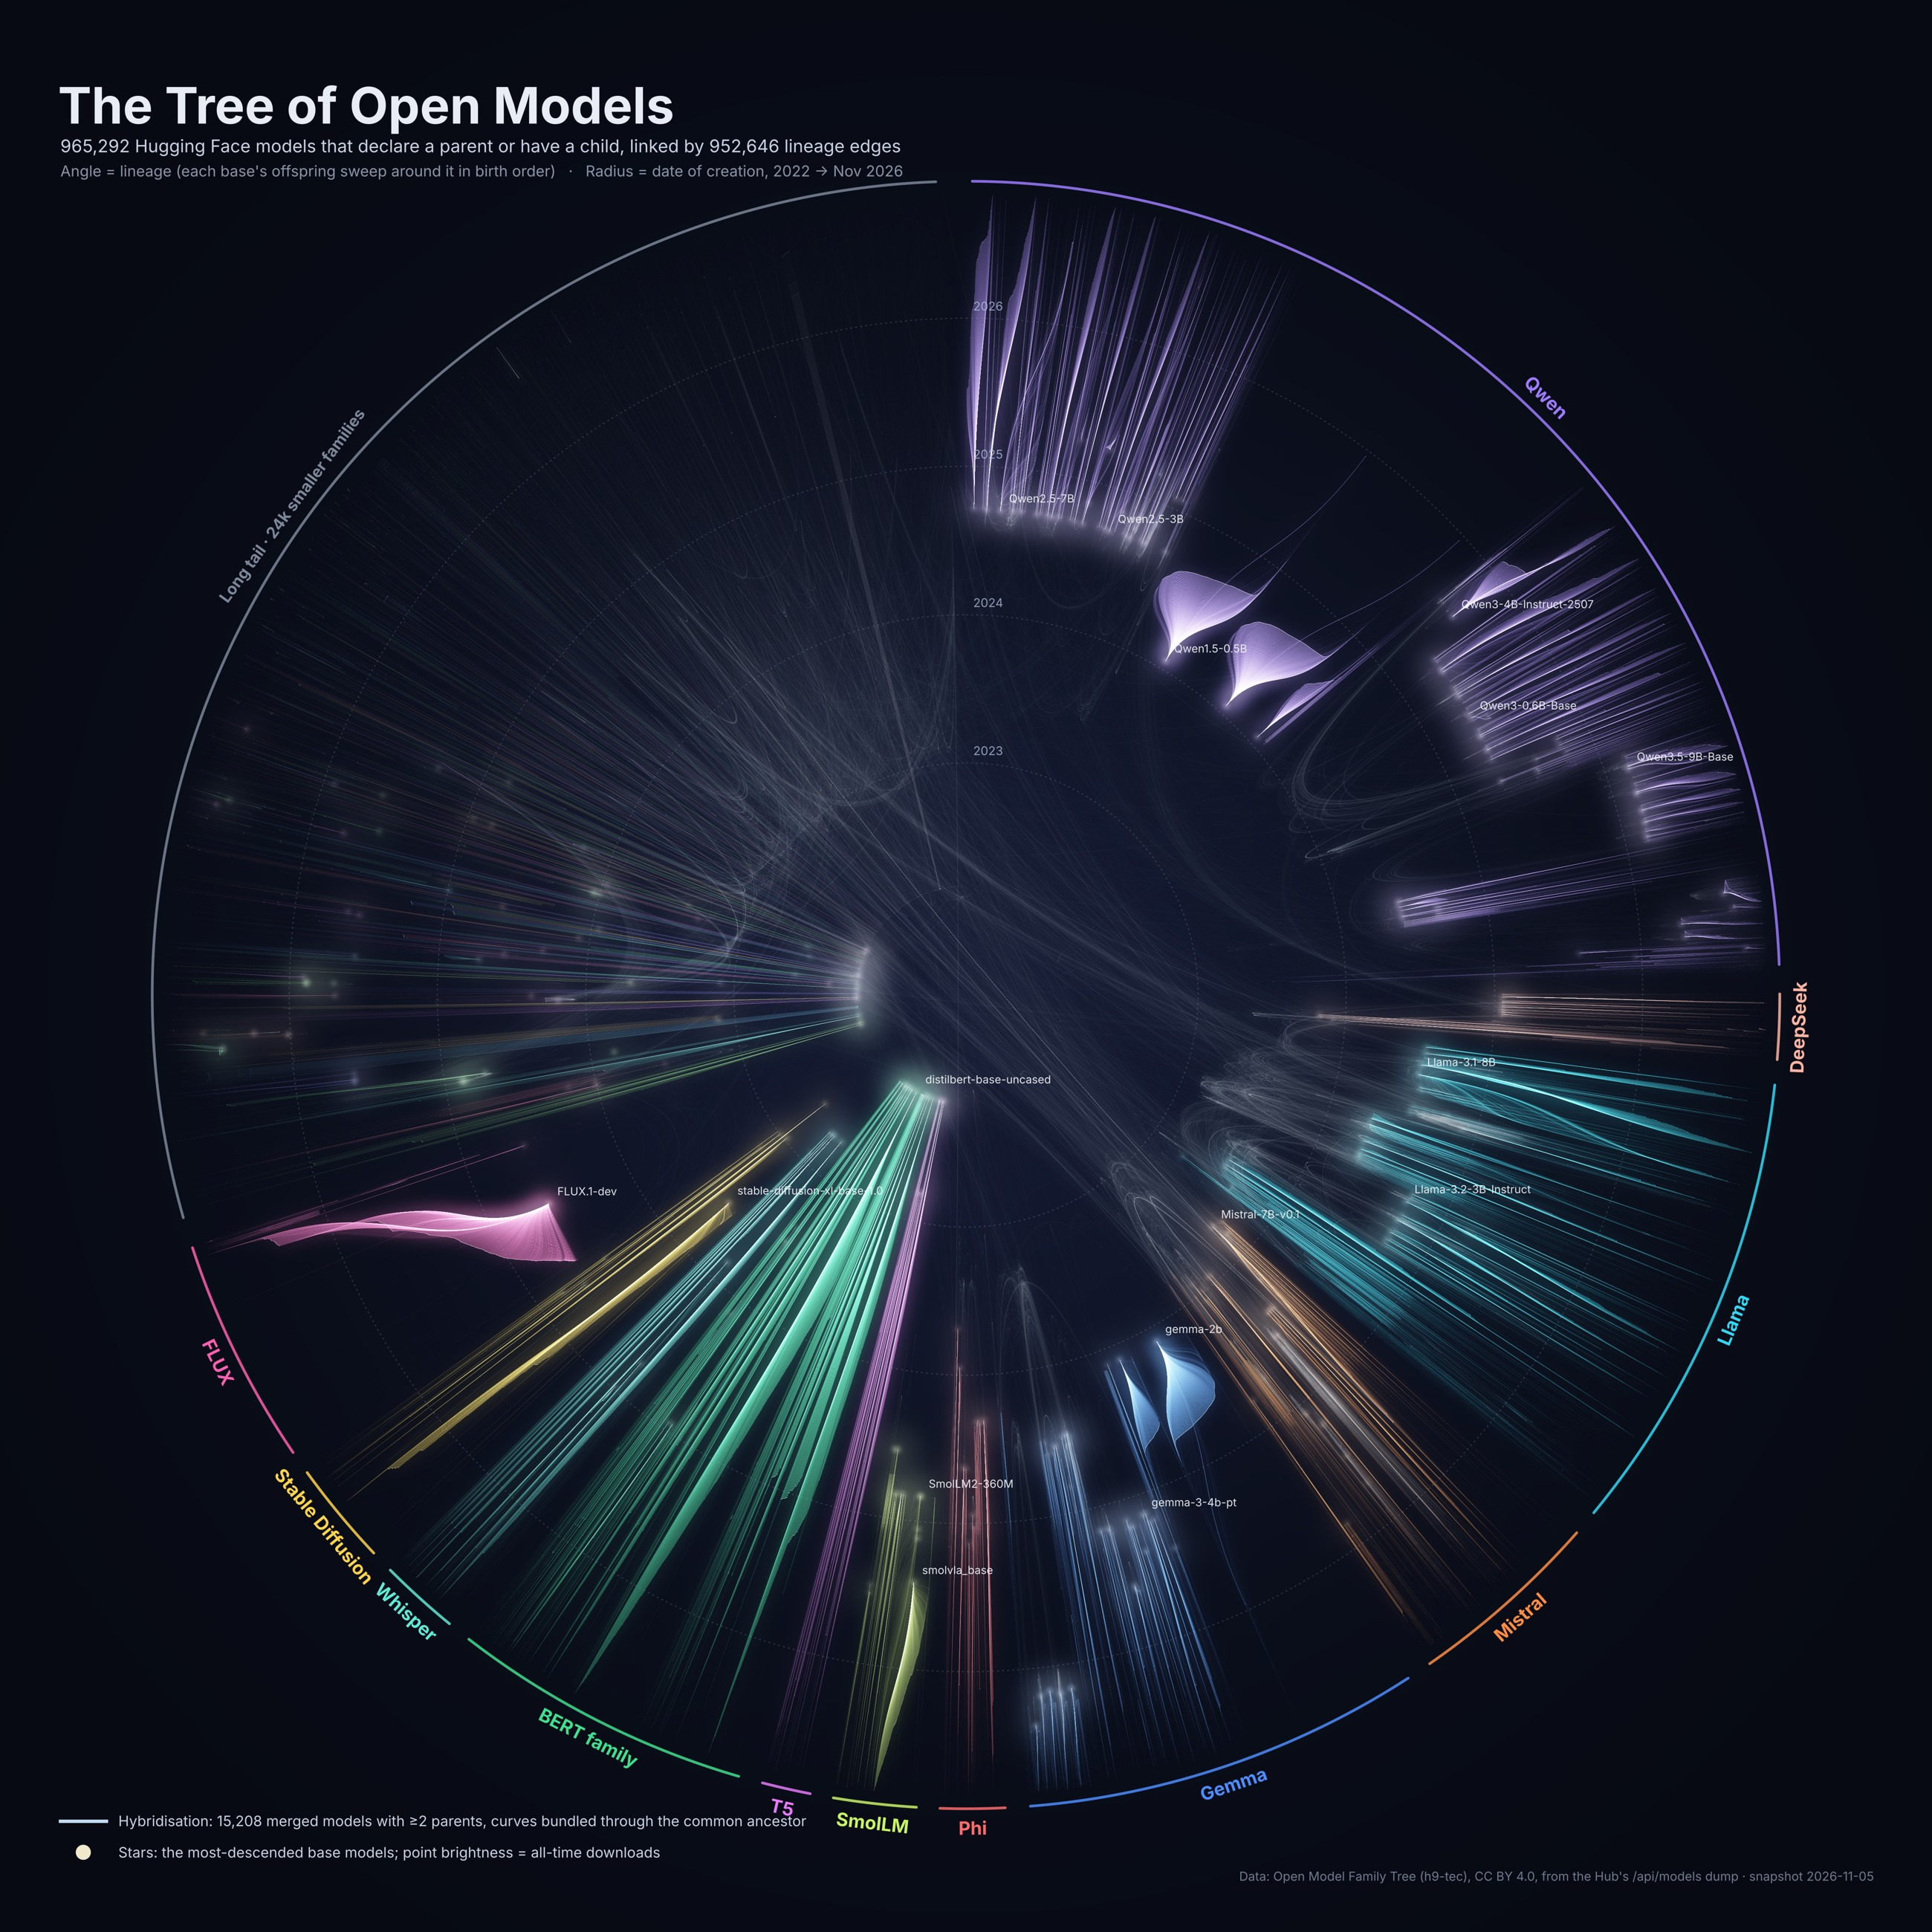
\includegraphics[width=\textwidth]{figs/f1.jpg}
\caption{\textbf{The Tree of Open Models.} Every Hugging Face model that declares a parent or has a child (\nConnected models). Radius encodes the creation date, from the inner ring (early 2022) to the rim (5 November 2026); dashed rings mark 1 January of each year. Angle encodes lineage: each super-family occupies a wedge, each root's descendants occupy an interval proportional to their number, and children are placed in birth order, so a base's offspring sweep around it as they appear. Curves follow the primary tree; pale bundled curves are the \nHybrids multi-parent merges, routed through the parents' common ancestor. Stars mark the most-descended bases; point brightness scales with all-time downloads. The bright ``sails'' are single bases with very large broods of offspring created in short bursts.}
\label{fig:hero}
\end{figure*}

\section{Lineage graph construction}\label{sec:graph}
\begin{itemize}\setlength{\itemsep}{1pt}
\item A \emph{root} is a model with descendants but no declared parent; there are \nRoots.
\item Every non-root has a \emph{primary parent}: its only parent or, for a multi-parent model, the parent with the largest lineage (ties broken by age). This rule differs from the first-listed parent for \nPrimaryChanged models. Primary parents define a spanning forest, the \emph{primary tree}; all other links are \emph{hybridisation} edges.
\item A model's \emph{generation} is its depth in the primary tree. Its \emph{hybrid depth} is the largest number of multi-parent events on any path from a root.
\item A \emph{family} is the set of models below one root in the primary tree. For reporting we also use the upstream series keys (\nFamilies keys, such as \texttt{qwen2.5} or \texttt{llama-3.1}) grouped into twelve \emph{super-families} (Qwen, Llama, Gemma, Mistral, FLUX, Stable Diffusion, BERT family, Whisper, SmolLM, DeepSeek, Phi and T5) plus a long tail.
\end{itemize}

\section{Methods}\label{sec:methods}
\paragraph{Structure (\RQ1).} Family size is the number of models in a root's primary subtree, root included. We fit a discrete power law above an $x_{\min}$ chosen by Kolmogorov--Smirnov minimisation and compare it with lognormal and exponential alternatives by normalised log-likelihood ratios $R$, where $R>0$ favours the power law \citep{clauset2009,alstott2014}. Concentration is summarised by the Gini coefficient and top shares.

\paragraph{Hybridisation (\RQ2).} For every multi-parent model, each pair of its parents is classified by declared ancestry as a \emph{backcross} (one parent descends from the other), \emph{siblings} (they share a direct parent), \emph{cousins} (they share a more distant ancestor) or an \emph{outcross} (no shared ancestor). The null model re-pairs parents at random 100 times, shuffling them across merged models while preserving each model's number of parents and each parent's frequency.

\paragraph{Tempo (\RQ3).} The lag of an edge is the child's creation time minus the parent's. We exclude ghost and backfilled endpoints and negative lags (\pctNegLag of the \nLagEdges eligible edges). A base's \emph{reaction time} for a relation is the lag of its first child of that kind; we compute it for the \nMajorBases bases with at least 100 direct children released between 1 January 2023 and six months before the snapshot, and test cohort trends with Spearman's $\rho$. Because declaring a base became common only gradually, we repeat the test for bases released from 2024 onwards.

\paragraph{Attention (\RQ4).} A derivative is \emph{active} if it was downloaded at least once in the 30 days before the snapshot. A logistic regression relates activity to relation type, generation, having several parents, uploader size and age (both $\log_{10}$), with super-family indicators and standard errors clustered by family key.

\paragraph{Speciation (\RQ5).} Pipeline tags are mapped to twelve task groups (for example text generation, vision--language, text classification, fill-mask, embeddings and ranking, image and video generation). An edge \emph{speciates} when parent and child fall in different groups; we use the \nTaskEdges edges where both tags are known.

\paragraph{Uncertainty and robustness.} Confidence intervals for proportions come from a cluster bootstrap with families as clusters (500 replicates) \citep{efron1993}. We re-run headline metrics under an alternative primary-parent rule, without quantised models, without the top 1\% of uploaders, and on the last 24 months only.

\paragraph{Visualisation.} The radial chronogram (Figure~\ref{fig:hero}) places each model at an angle given by a birth-ordered depth-first layout of its family and at a radius given by its creation date; links are cubic curves that leave and enter radially. Hybrid links are bundled through the position of the parents' most recent common ancestor. A custom additive rasteriser draws all \nEdges links with luminous blending. The coral view (Figure~\ref{fig:coral}) lays out the skeleton of models that have children with a force-directed algorithm and arranges childless offspring around their parent on sunflower discs.

\section{Results}
\subsection{Structure (\RQ1)}
Lineage is concentrated in a few giant families. \pctRootsSmall of roots have families of at most three models, yet the top 1\% of roots (\nTopOnePctRoots) hold \pctTopOnePctRoots of all connected models and the ten largest alone hold \pctTopTenRoots. The Gini coefficient of family sizes is \giniFamily, and the largest single-root family has \familyMax models. The tail is heavy: a power law with $\alpha=\plAlpha$ fits sizes above $x_{\min}=\plXmin$ (\plNtail roots) and is strongly preferred to an exponential ($R=\plExR$, $p$\,\plExP), but cannot be distinguished from a lognormal ($R=\plLnR$, $p=\plLnP$; Figure~\ref{fig:stats}a). By named lineage, the Qwen super-family alone contains \nQwenSuper models (\pctQwenSuper of the graph), and the ten largest family keys hold \pctTopTenKeys.

The tree is shallow and bushy. \pctDepthOne of derivatives are direct children of a root and only \pctDepthThree sit three or more generations deep; the 99th percentile is \depthPnn generations and the maximum is \depthMax in the primary tree, or \ldepthMax along the longest path through merges. The median parent has \outdegMedian children, while the most prolific has \outdegMax. Overall \pctLeaves of derivatives are leaves, but fertility depends sharply on the relation: \pctLeafAdapter of adapters and \pctLeafQuantized of quantisations never have children, against \pctLeafFinetune of fine-tunes and only \pctLeafMerge of merges. Merges are the ecosystem's breeding stock. Table~\ref{tab:gen} shows that adapters dominate the first generation, while fine-tunes and quantisations dominate later ones. Finally, \nUnderGhost models (\pctUnderGhost) descend from ghost roots, lineages whose founder is no longer public.

\begin{table}[t]
\centering\small
\caption{Relation of each derivative to its primary parent, by generation.}
\label{tab:gen}
\resizebox{\columnwidth}{!}{\begin{tabular}{lrrrrr}
\toprule
Generation & Models & Fine-tune & Adapter & Quantised & Merge \\
\midrule
1 & 607{,}233 & 38.6\% & 44.3\% & 16.3\% & 0.8\% \\
2 & 191{,}813 & 43.6\% & 26.2\% & 27.9\% & 2.3\% \\
3 & 82{,}510 & 40.3\% & 19.2\% & 36.4\% & 4.1\% \\
4+ & 37{,}886 & 42.0\% & 7.4\% & 42.7\% & 7.8\% \\
\bottomrule
\end{tabular}
}
\end{table}

\begin{figure}[t]
\centering
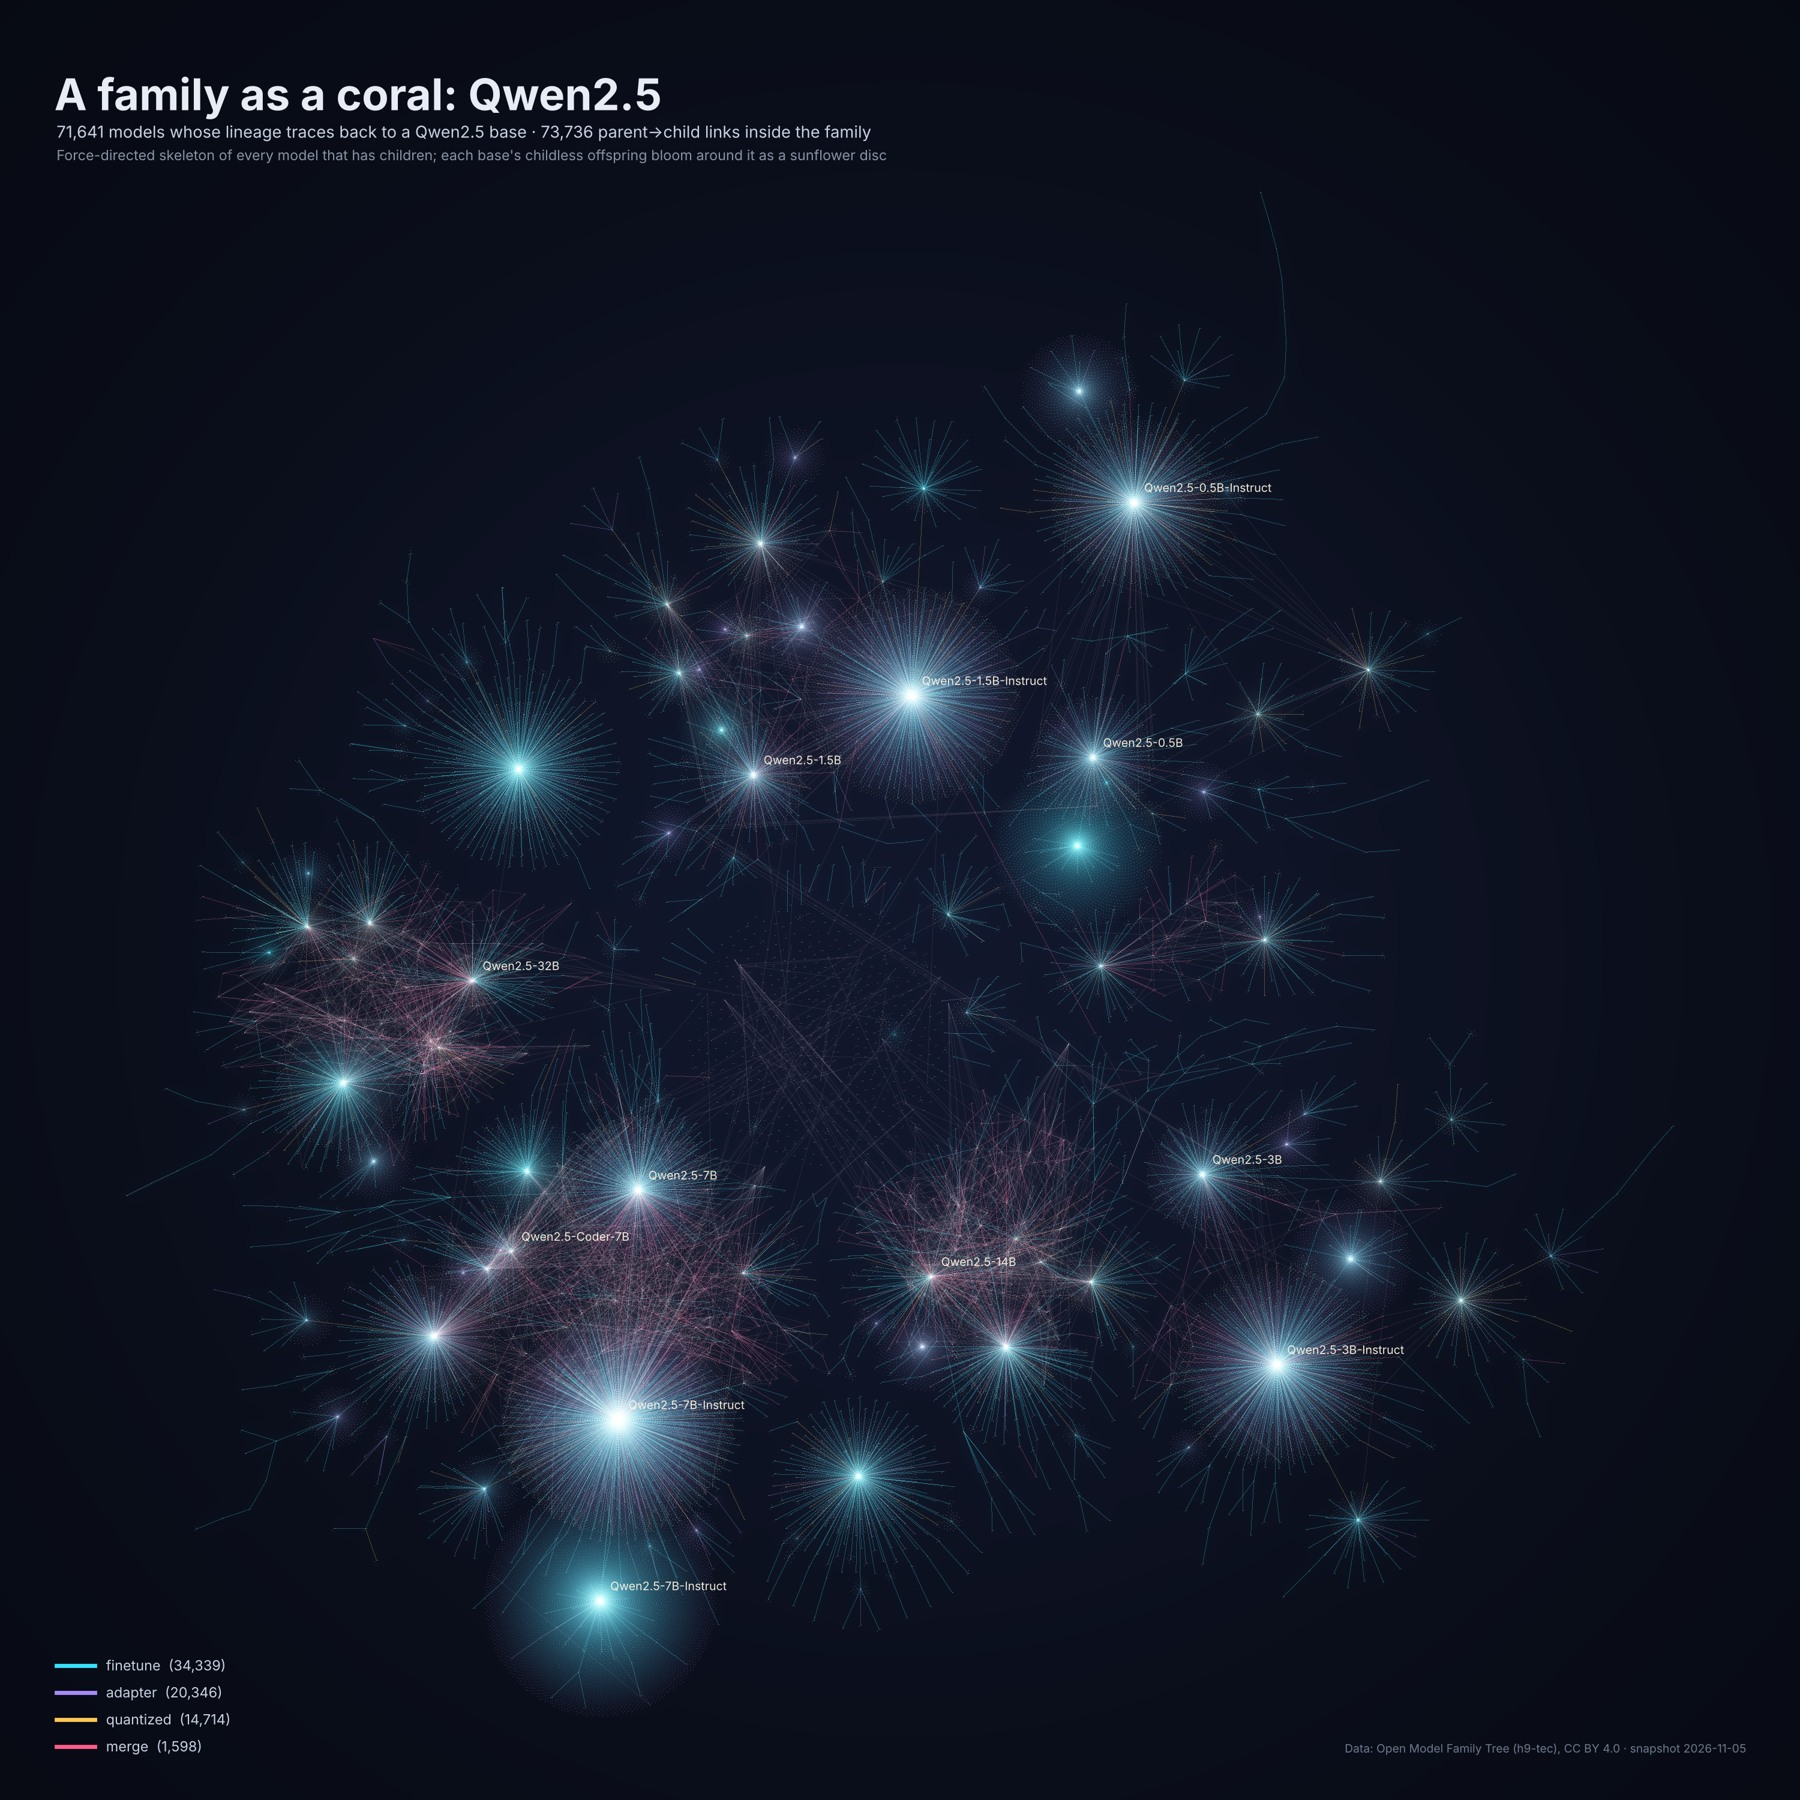
\includegraphics[width=\columnwidth]{figs/f2.jpg}
\caption{\textbf{A family as a coral: Qwen2.5} (\nQwenTwoFive models). The force-directed skeleton holds every model that has children; childless offspring bloom around their parent on sunflower discs, ordered by relation (colour) and birth. Bright hubs are the base and instruct checkpoints with the most direct children.}
\label{fig:coral}
\end{figure}

\subsection{Hybridisation (\RQ2)}
\nHybrids models declare two or more parents, including \pctMergeMulti of those labelled as merges. Most hybrids have two parents (\pctTwoParents), but one lists \maxParents. Across \nPairs parent pairs, \pctBackcross are backcrosses, \pctSibling siblings and \pctCousin cousins, while \pctOutcross share no declared ancestor (95\% CI \outcrossLo--\outcrossHi). Under random re-pairing only \pctNullRelated of pairs are related, so merges join relatives \assortRatio times more often than chance (permutation $p\le\permP$; Figure~\ref{fig:hybrid}). Family keys tell the same story: \pctCrossFamily of observed pairs cross family keys, against \pctNullCross under the null, and \pctCrossSuper cross super-families.

Merging also builds the deepest lineages. One chain reaches \hybDepthMax successive merges. Of the \nDeepHybrid models that sit at least ten merges deep, \pctDeepTopAuthor come from a single account (\nDeepAuthors accounts in total), and \pctDeepTopAuthorQuant of its models at that depth are quantisations rather than merges. The \nDeepMulti multi-parent models at that depth come from \nDeepMultiAuthors accounts, and the largest of these contributes \pctDeepMultiTopAuthor. The largest ancestor set of a merged model contains \ancMax models.

\begin{figure*}[t]
\centering
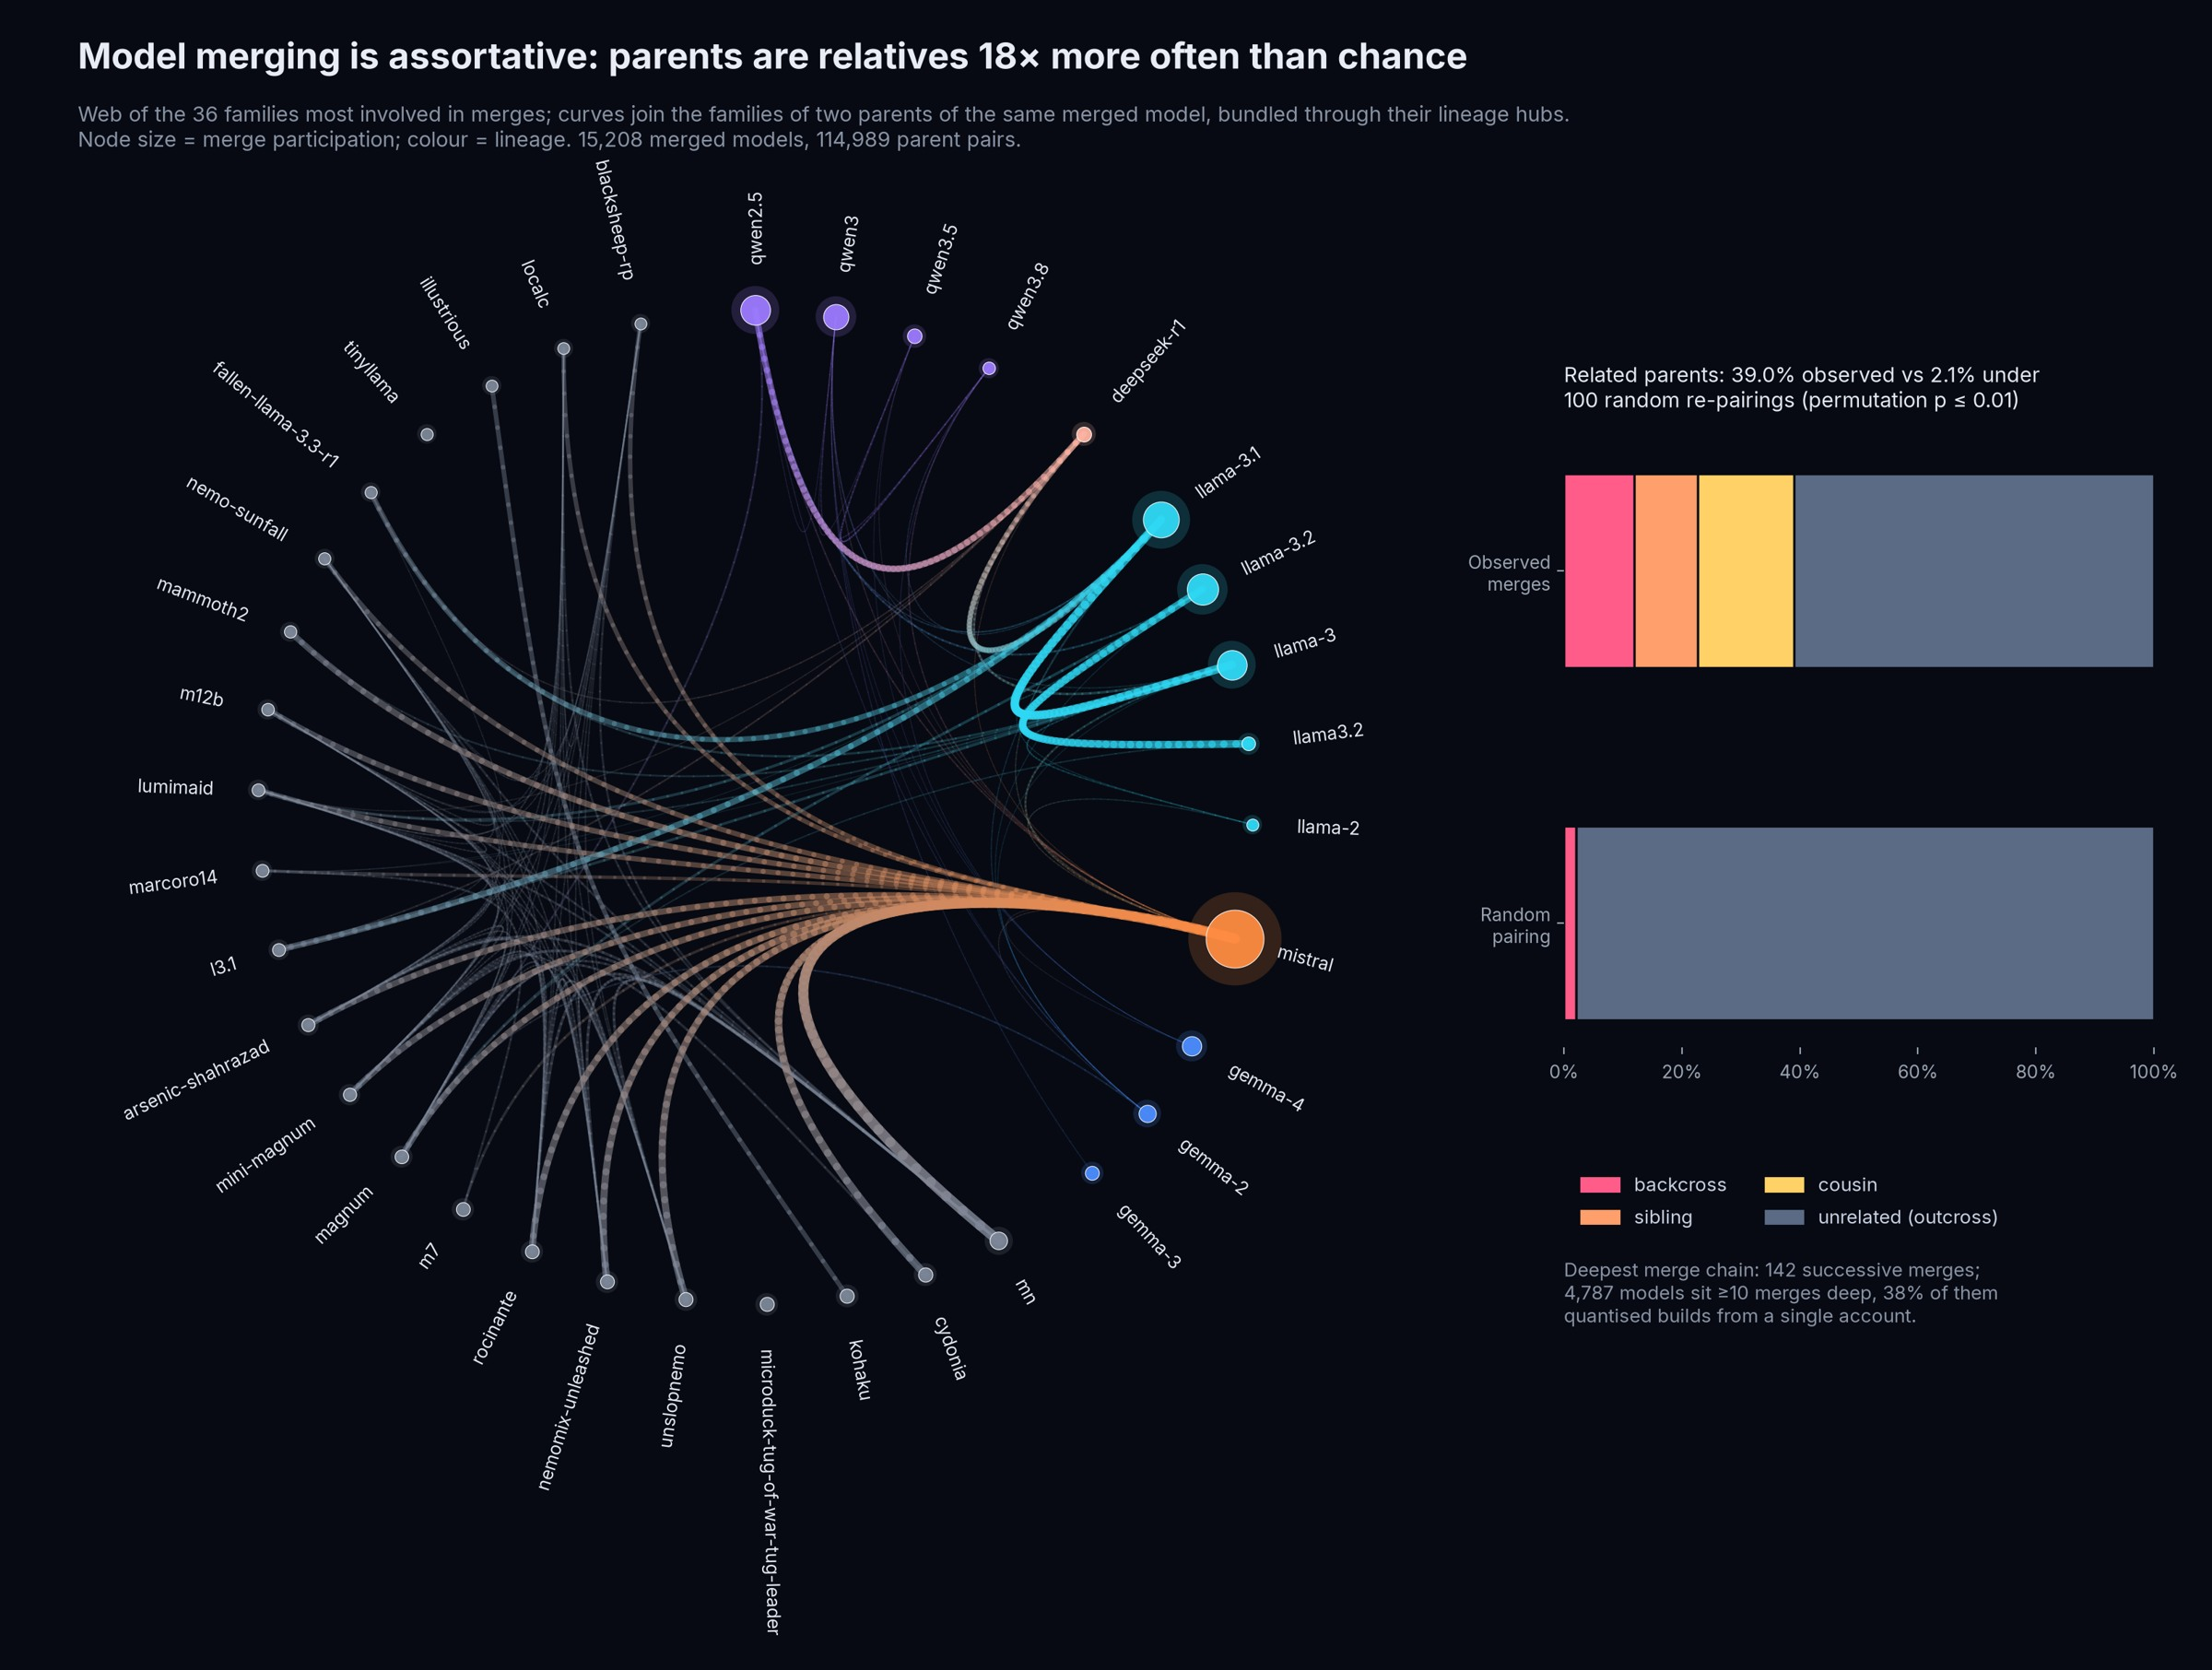
\includegraphics[width=0.94\textwidth]{figs/f5.jpg}
\caption{\textbf{Model merging is assortative.} Left: the families most involved in merges; curves join the families of two parents of the same merged model, bundled through their super-family hubs. Right: kinship of the \nPairs parent pairs compared with 100 random re-pairings.}
\label{fig:hybrid}
\end{figure*}

\subsection{Tempo (\RQ3)}
Derivative production exploded after 2023 (Figure~\ref{fig:stream}). The graph gained \birthsTwentyThree derivatives in 2023, \birthsTwentyFour in 2024, \birthsTwentyFive in 2025 and \birthsTwentySix in the first ten months of 2026. The busiest month, \birthsPeakMonth, added \birthsPeakCount derivatives, led by the \peakSuper super-family; no single account contributed more than \pctPeakTopUploader of them.

\begin{figure*}[t]
\centering
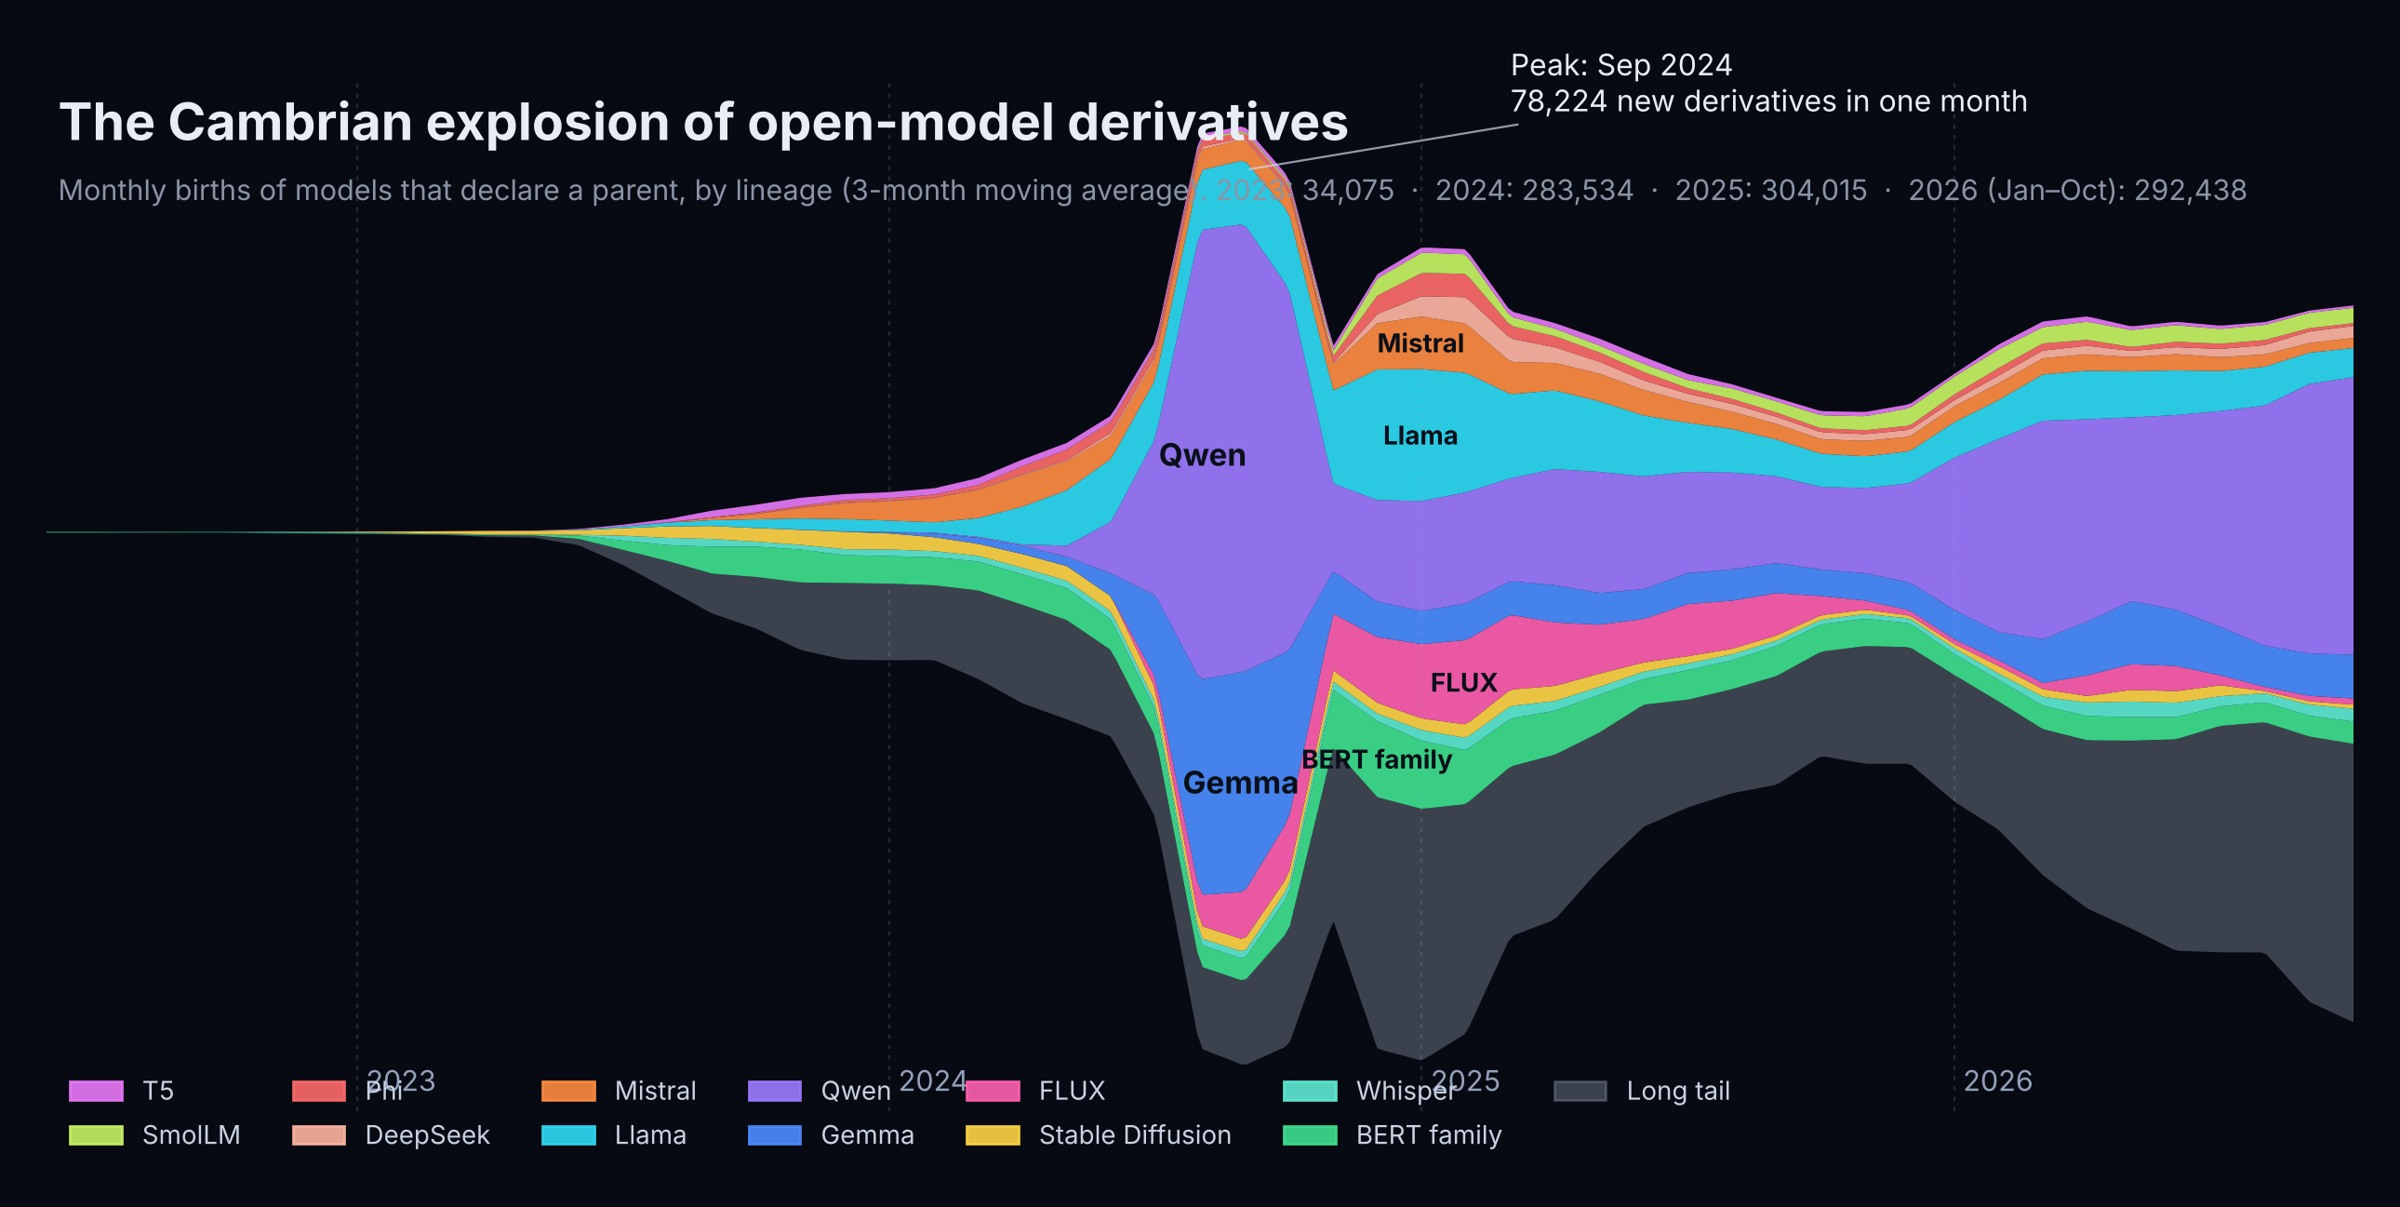
\includegraphics[width=\textwidth]{figs/f4.jpg}
\caption{\textbf{The Cambrian explosion of open-model derivatives.} Monthly births of models that declare a parent, by super-family (3-month moving average, streamgraph layout).}
\label{fig:stream}
\end{figure*}

Quantisations follow their parent fastest: the median lag is \lagQuantized days, \pctQuantDay arrive within a day, \pctQuantWeek within a week and \pctQuantMonth within a month. Merges follow with a median of \lagMerge days (\pctMergeMonth within a month). Fine-tunes (\lagFinetune days) and adapters (\lagAdapter days) have long lags because popular bases keep attracting derivatives for years (Figure~\ref{fig:stats}b).

For the \nMajorBases heavily reused bases, the median reaction time is \rtQuantAll days for the first quantisation, \rtFinetuneAll for the first fine-tune, \rtAdapterAll for the first adapter and \rtMergeAll for the first merge. Reaction keeps getting faster (Table~\ref{tab:reaction}, Figure~\ref{fig:stats}c). The median time to the first fine-tune fell from \rtFinetuneEarly days for bases released in the second half of 2023 to \rtFinetuneLate days in the first half of 2026; for quantisations it fell from \rtQuantEarly to \rtQuantLate days, and for adapters from \rtAdapterEarly to \rtAdapterLate. Release date and reaction time are negatively correlated for fine-tunes ($\rho=\rhoFinetuneAll$; $\rho=\rhoFinetune$ for the \nRhoFinetune bases released from 2024), quantisations ($\rho=\rhoQuantAll$; $\rho=\rhoQuant$ for \nRhoQuant bases from 2024) and adapters ($\rho=\rhoAdapter$ from 2024), but not for merges ($\rho=\rhoMerge$, $p=\pRhoMerge$).

\begin{table}[t]
\centering\small
\caption{Median days from a base's release to its first child of each kind, by release cohort (bases with at least 100 direct children).}
\label{tab:reaction}
\resizebox{\columnwidth}{!}{\begin{tabular}{lrrrrr}
\toprule
Cohort & Bases & Fine-tune & Quantised & Adapter & Merge \\
\midrule
2023H1 & 32 & 165.2 & 203.4 & 315.0 & 1263.4 \\
2023H2 & 91 & 35.1 & 13.6 & 35.0 & 146.1 \\
2024H1 & 138 & 17.7 & 12.8 & 58.8 & 27.0 \\
2024H2 & 180 & 5.4 & 5.9 & 44.1 & 20.7 \\
2025H1 & 127 & 4.1 & 3.9 & 18.7 & 22.9 \\
2025H2 & 68 & 3.1 & 4.0 & 16.6 & 23.9 \\
2026H1 & 65 & 2.8 & 2.8 & 8.2 & 42.3 \\
\bottomrule
\end{tabular}
}
\end{table}

Fast reaction does not mean short attention. For the \nDecayBases bases older than a year, the median share of first-year children born in the first 30 days is only \pctFirstMonth, and half of a base's first-year children typically arrive after \halfLife days. Production is also concentrated among uploaders: of \nUploaders accounts, the top ten produce \pctTopTenUploaders of all derivatives, the top hundred \pctTopHundredUploaders and the top 1\% (\nTopUploaders accounts) \pctTopUploaders, a Gini coefficient of \giniUploaders.

\subsection{Attention (\RQ4)}
Downloads are even more concentrated than reproduction. Derivatives have accumulated \totalChildDownloads downloads, \pctTopDownloads of them by the top 1\% of derivatives (Gini \giniDownloads). Median all-time downloads are \dlQuantized for quantisations, \dlMerge for merges, \dlFinetune for fine-tunes and \dlAdapter for adapters. \pctDormant of derivatives had no download in the last 30 days (95\% CI \dormantLo--\dormantHi) and \pctZeroAll were never downloaded. Dormancy reaches \pctDormantFinetune among fine-tunes, against \pctDormantAdapter for adapters, \pctDormantQuantized for quantisations and \pctDormantMerge for merges.

The regression (n\,=\,\nLogit, pseudo-$R^2$\,=\,\pseudoRsq; Figure~\ref{fig:stats}d) confirms the ranking. Relative to fine-tunes, the odds of being active are \orQuant times higher for quantisations (95\% CI \orQuantLo--\orQuantHi), \orAdapter for adapters and \orMerge for merges. They fall with generation (\orGenTwo for generation two, \orGenThree for three or more) and rise with uploader size (\orAuthor per tenfold) and age (\orAge per tenfold); having several parents has no clear effect (\orHybrid, CI \orHybridLo--\orHybridHi).

Within the \nBigFamilies families with at least 50 descendants, descendants collect a median \pctDescShare of the family's downloads, and in \pctOutgrow of families at least one child out-downloads its root. Reproduction and use are related but not aligned: the rank correlation between a parent's number of children and its downloads is \rhoKids among \nRhoKids parents with at least ten children, and \pctAdapterDominated of the \nBasesHundred bases with at least 100 children owe 90\% or more of them to adapters.

\begin{figure*}[t]
\centering
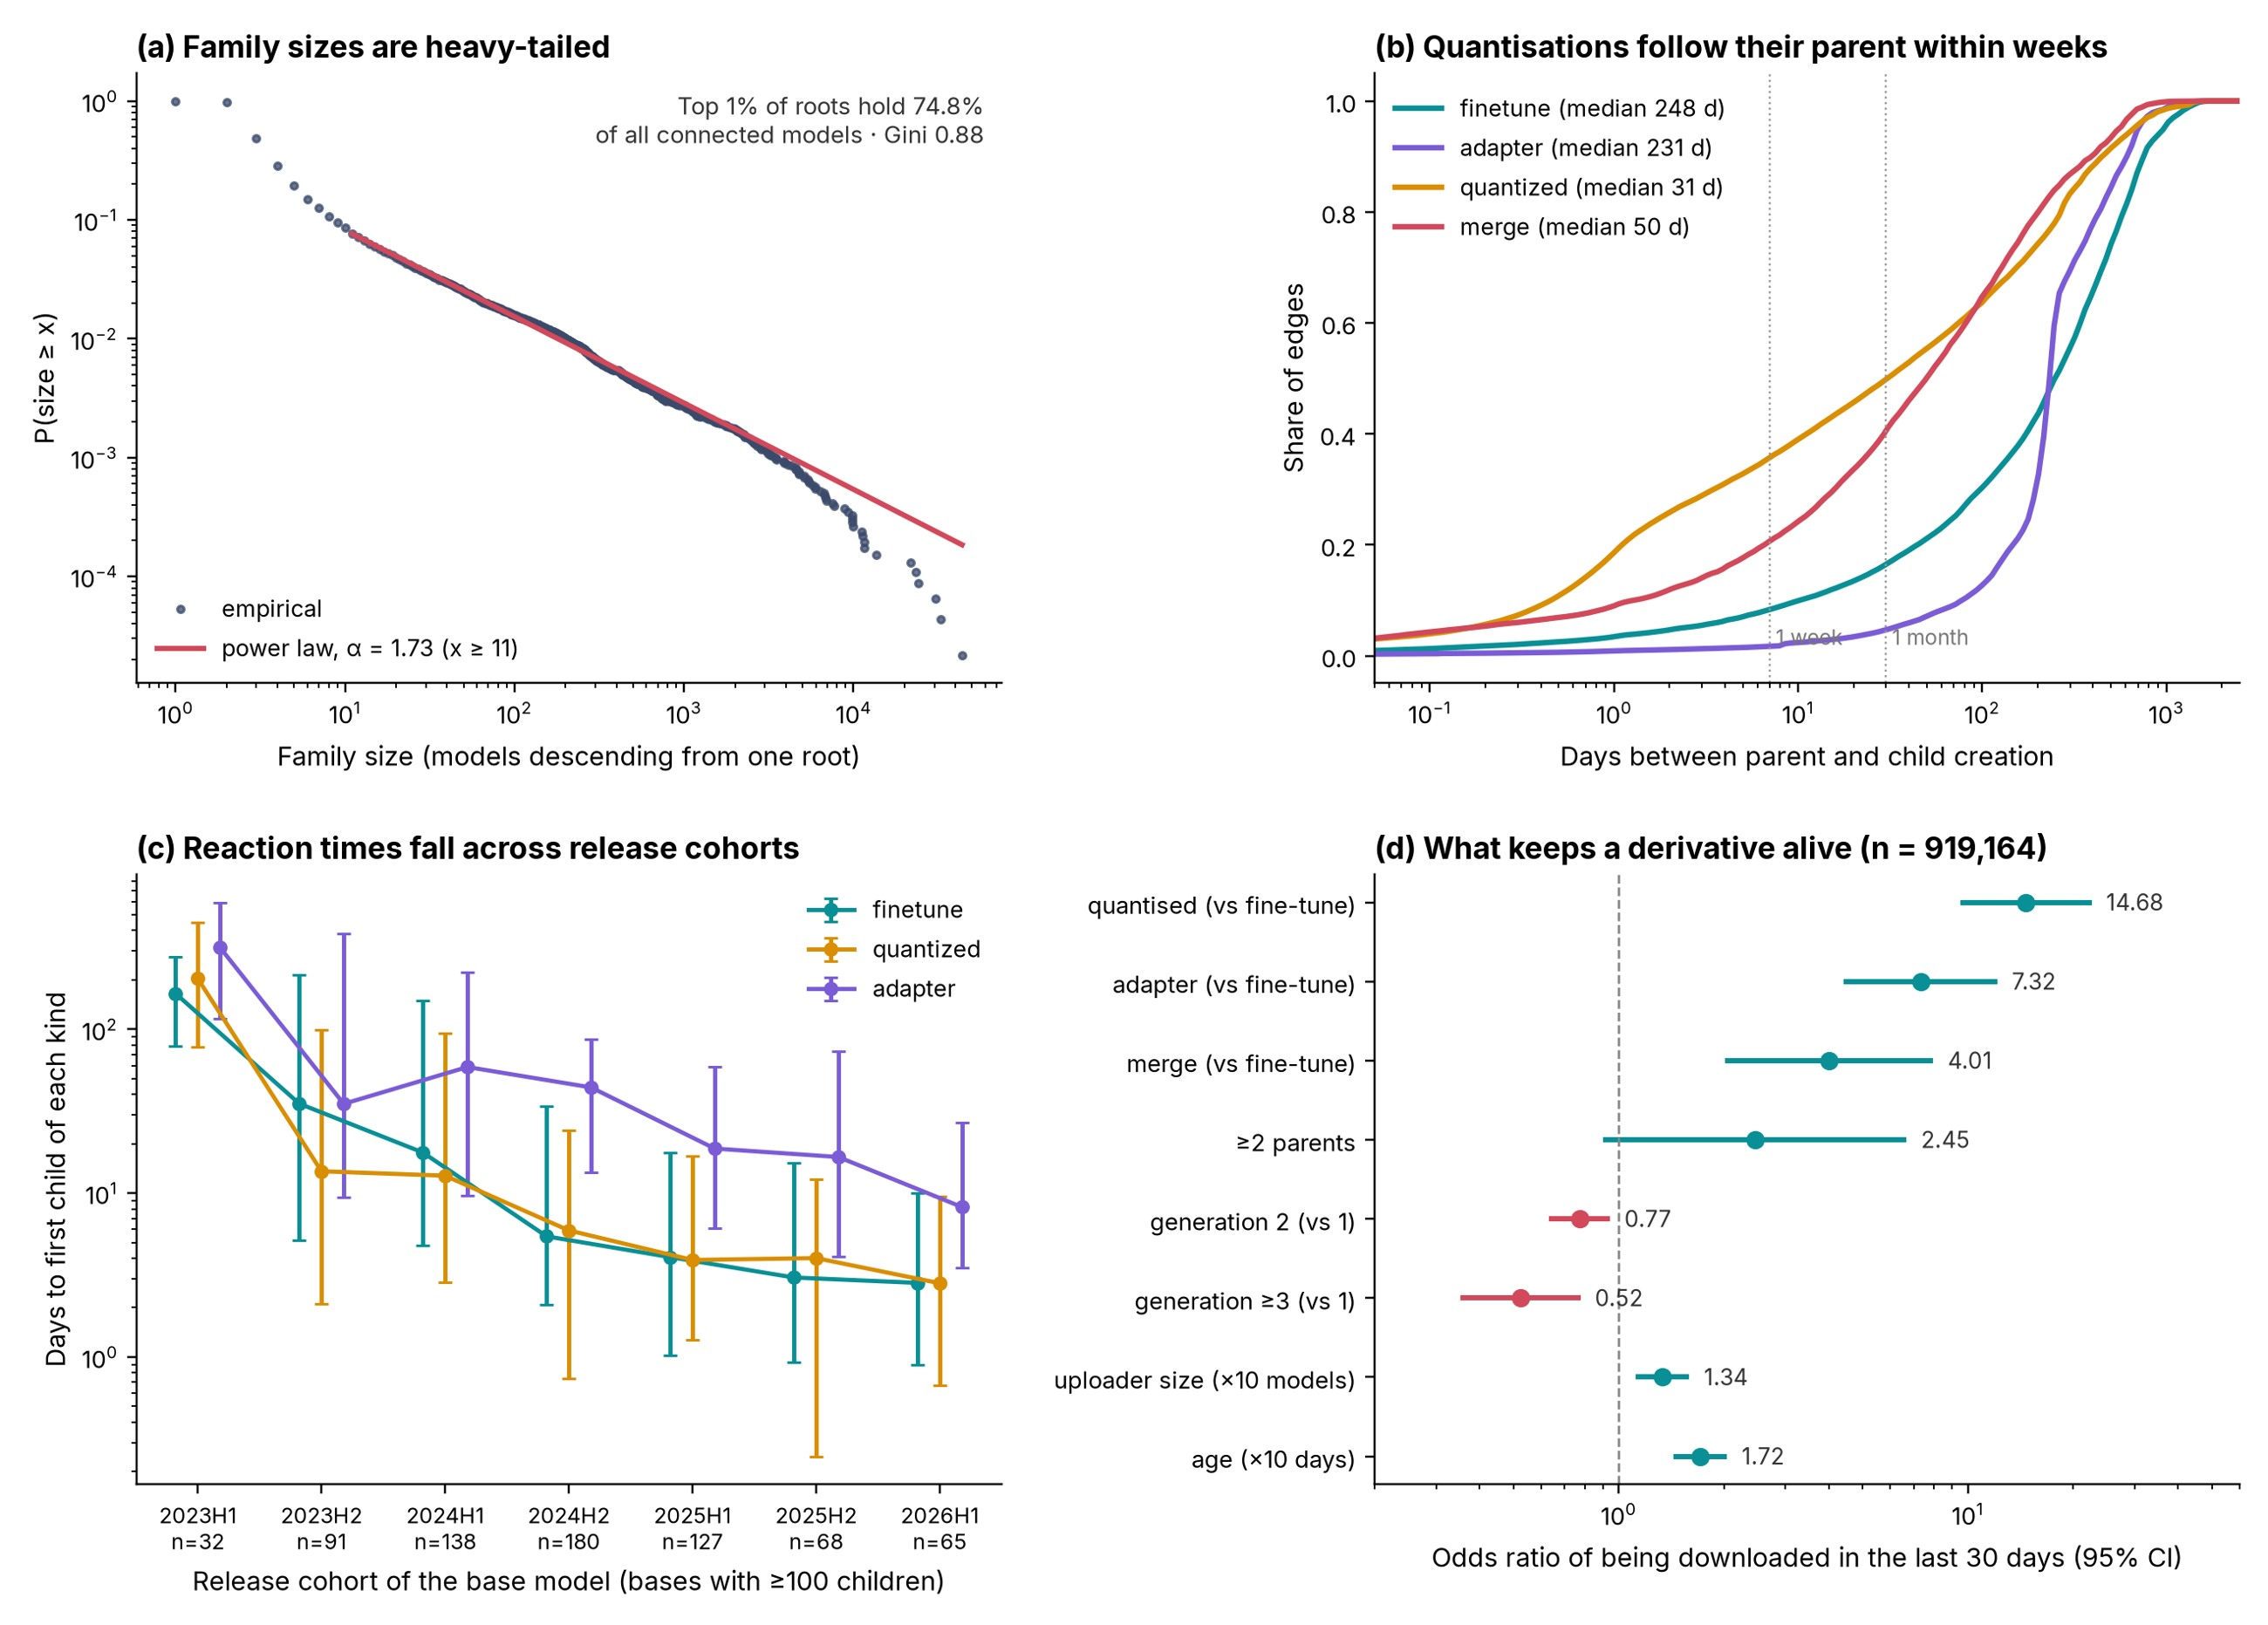
\includegraphics[width=0.96\textwidth]{figs/f6.jpg}
\caption{\textbf{Statistics.} (a) Complementary CDF of family sizes with the fitted power law. (b) Cumulative distribution of the parent-to-child lag by relation. (c) Median reaction time by release cohort with interquartile ranges. (d) Odds ratios of being downloaded in the last 30 days (super-family indicators omitted from the plot).}
\label{fig:stats}
\end{figure*}

\subsection{Speciation (\RQ5)}
Of the \nTaskEdges edges whose two endpoints have a known task, \pctSpeciation cross a task group (95\% CI \specLo--\specHi), and \pctPipelineChange change the exact pipeline tag (Figure~\ref{fig:chord}). Fine-tunes speciate most (\pctSpecFinetune), followed by quantisations (\pctSpecQuantized) and adapters (\pctSpecAdapter); merges rarely do (\pctSpecMerge). The single largest route is fill-mask to text classification (\nFillMaskClass edges, \pctTopTransition of all pipeline changes), followed by vision--language to text generation (\nVlmText) and fill-mask to token classification (\nFillMaskToken). By parent task, \pctSpecFillMask of edges from fill-mask models change task and \pctSpecEmbed from embedding and ranking models, against \pctSpecTextGen for text generation and \pctSpecImageGen for image and video generation: generative lineages rarely speciate. Formats migrate too: \pctLibChange of the \nQuantLib quantised edges with known libraries change library, led by Transformers to MLX (\nToMlx) and to GGUF (\nToGguf).

\begin{figure}[t]
\centering
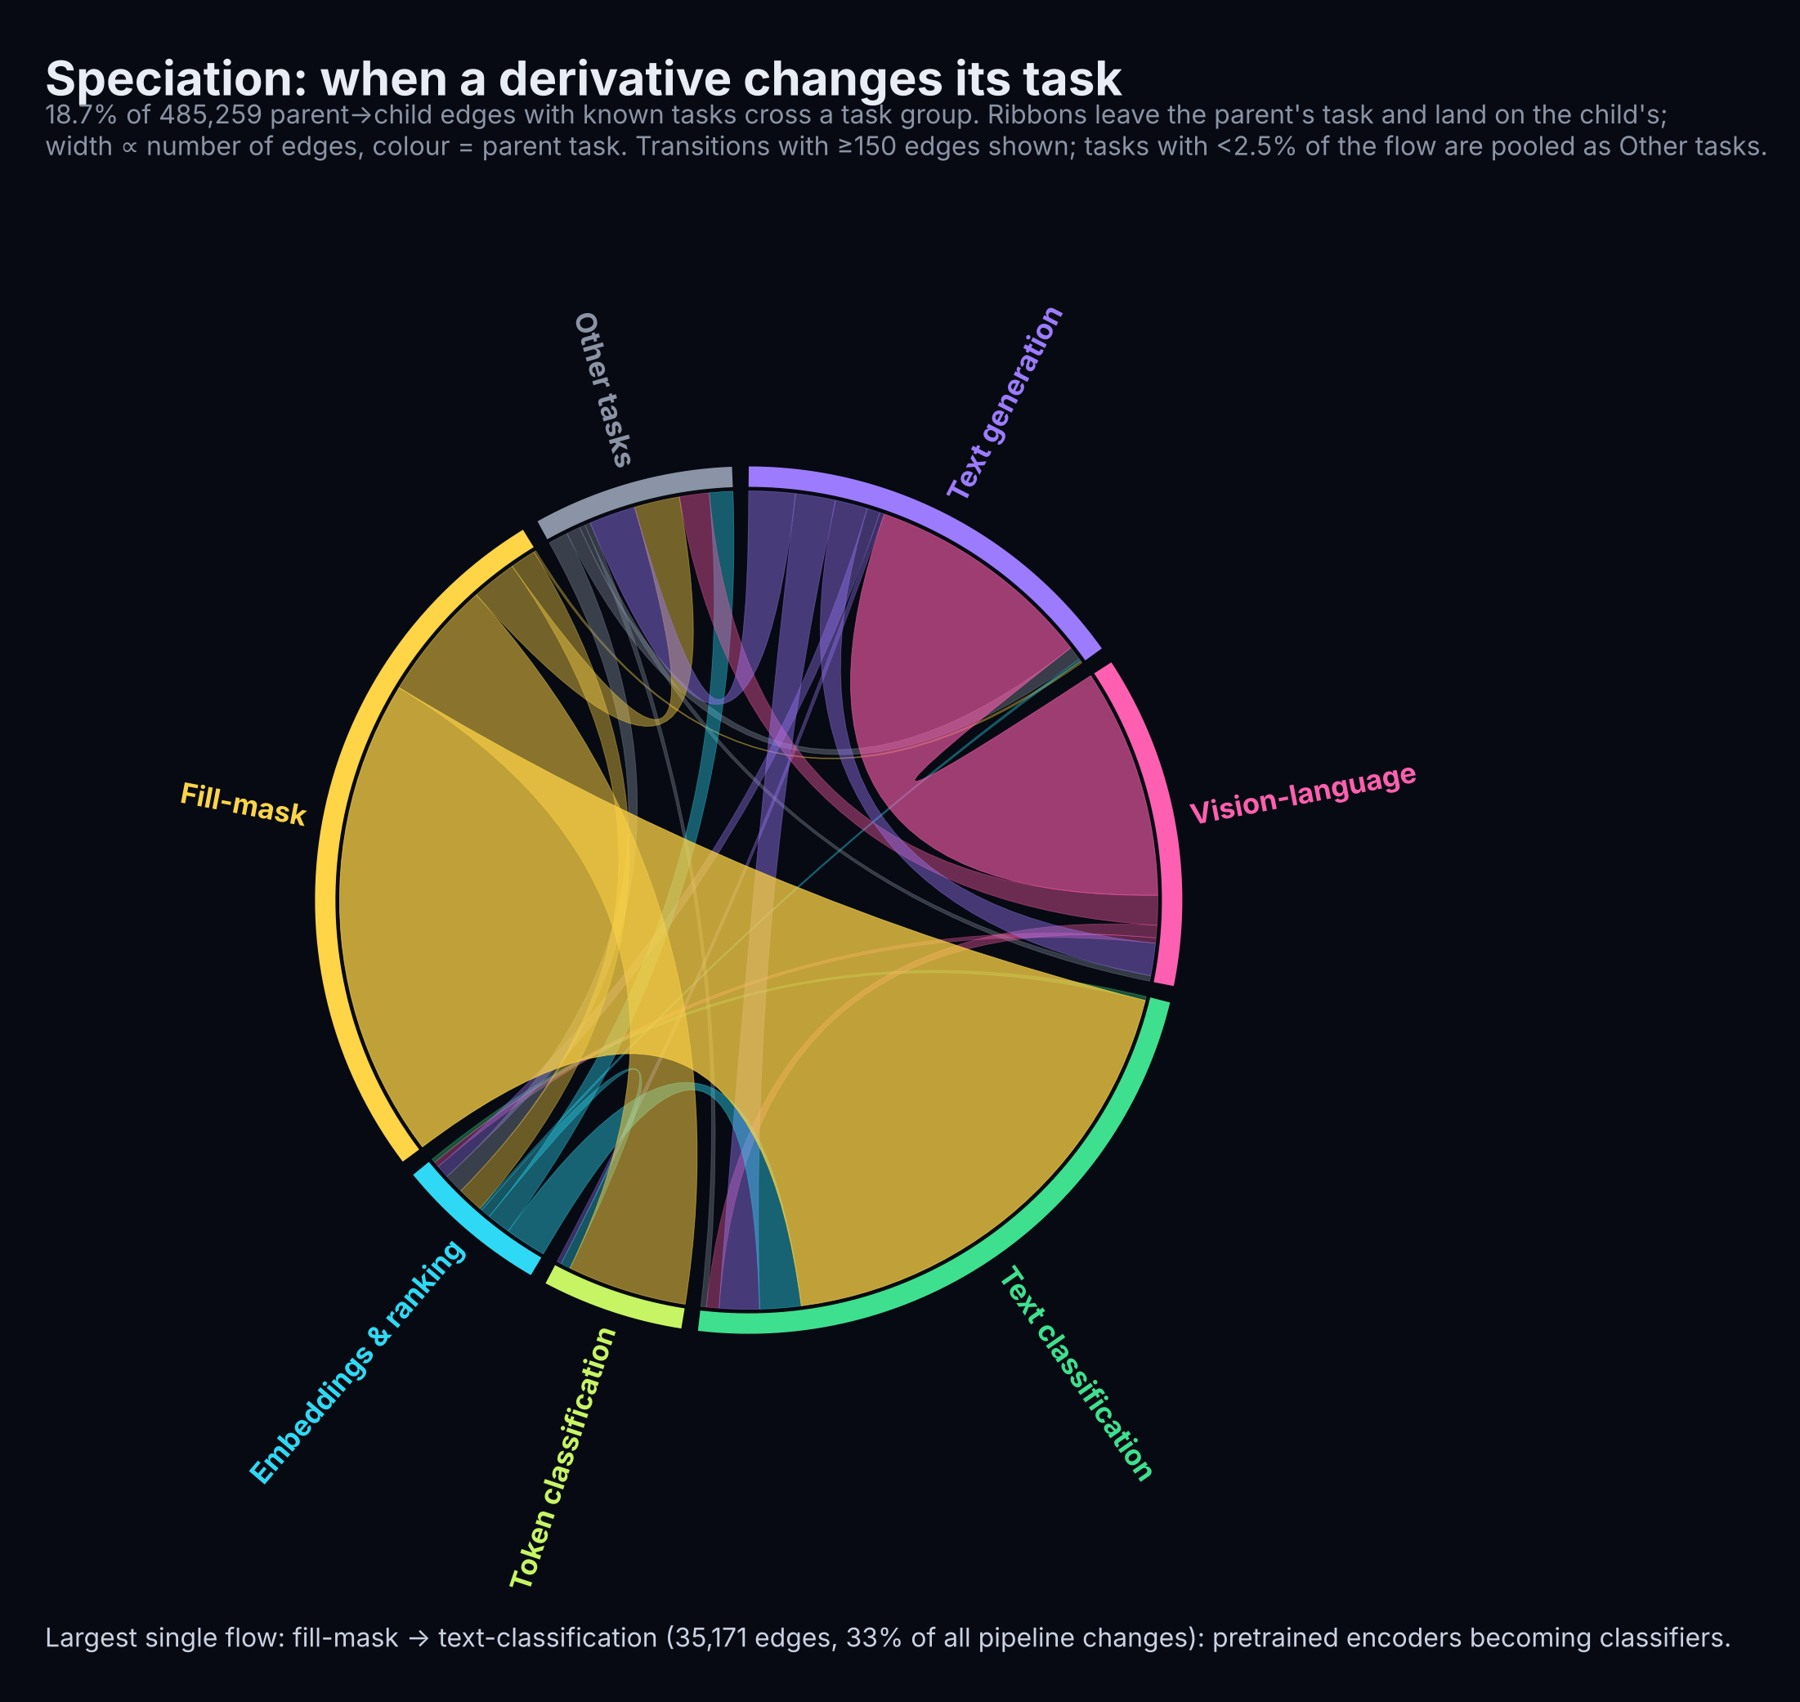
\includegraphics[width=\columnwidth]{figs/f3.jpg}
\caption{\textbf{Speciation.} Task changes along parent--child edges; ribbons leave the parent's task and land on the child's, with width proportional to the number of edges.}
\label{fig:chord}
\end{figure}

\subsection{Robustness}
Table~\ref{tab:robust} repeats five headline metrics under four alternative specifications. Concentration, speciation and dormancy stay of the same order in every case, and the first-listed parent rule leaves them almost unchanged.

\begin{table}[t]
\centering\small
\caption{Headline metrics under alternative specifications: Gini and top-10 share of family sizes, speciation rate, median fine-tune lag (days) and dormant share. Family metrics here count families of at least two models, so the top-10 share differs slightly from the value in the text.}
\label{tab:robust}
\resizebox{\columnwidth}{!}{\begin{tabular}{lrrrrr}
\toprule
Specification & Gini & Top-10 & Speciation & Lag (d) & Dormant \\
\midrule
Main specification & 0.88 & 23.3\% & 18.7\% & 247.6 & 12.4\% \\
First-listed primary parent & 0.88 & 23.1\% & 18.7\% & 247.6 & 12.4\% \\
Without quantised models & 0.92 & 28.7\% & 20.4\% & 247.6 & 15.1\% \\
Without top 1\% uploaders & 0.88 & 21.1\% & 22.4\% & 229.7 & 17.6\% \\
Last 24 months only & 0.86 & 20.8\% & 17.6\% & 275.6 & 15.0\% \\
\bottomrule
\end{tabular}
}
\end{table}

\section{Discussion}
\paragraph{A few bases carry the ecosystem.} With \pctTopOnePctRoots of all connected models below the top 1\% of roots, an evaluation, audit or safety fix applied to a handful of bases reaches most of the Hub's derivatives, and a defect in one of them propagates just as far. Lineage metadata is what makes such propagation traceable.

\paragraph{Derivatives arrive in days.} Fine-tunes and quantisations of a major release now appear within days, and reaction times have fallen across release cohorts. Release processes, evaluations and responsible-use guidance should assume that derivatives exist almost immediately; quantisers act as distribution infrastructure, and their builds have the highest median downloads of any relation.

\paragraph{Merging favours relatives, and its deepest chains are concentrated.} Merges join relatives far more often than chance, although most parent pairs (\pctOutcross) still share no declared ancestor. Chains reach \hybDepthMax merges deep, and most of the deepest multi-parent models come from a small number of accounts. Such chains make provenance hard to reason about without tooling, and license and safety obligations may be easier to lose along them.

\paragraph{Speciation follows architecture.} Fill-mask encoders are starting points that are almost always re-purposed, while generative models are mostly specialised within their task. Vision--language bases routinely give rise to text-only descendants.

\paragraph{Implications for platforms.} Platforms could validate declarations at upload (cycles, children older than their parents), surface ghost parents, rank search results with lineage-aware signals, and propagate notices such as deprecations or vulnerability reports down a lineage.

\section{Threats to validity}\label{sec:threats}
\paragraph{Construct.} We observe declared ancestry only: \pctDeclare of models declare a parent, so all counts are lower bounds, and relation labels may be inferred or wrong. Family keys rely on a naming heuristic. Download counts follow the Hub's counting conventions and include automated traffic.
\paragraph{Internal.} Creation time is not release time, the earliest dates are backfilled, and \pctNegLag of lags are negative. The acceleration of reaction times could partly reflect the adoption of declarations; restricting the test to bases released from 2024 onwards preserves the trend.
\paragraph{External.} We study one platform at one point in time through a third-party rebuild of its metadata; our reconstruction applies its own cleaning rules and may differ slightly from the upstream summaries.

\section{Ethics, limitations and future work}\label{sec:ethics}
We use public metadata only, report individual accounts anonymously, and make no judgement about the legality of any model. The main limitation is the missing license metadata, which prevented the license-drift analysis of our original design. That analysis would map each declared license to a class (permissive, copyleft, use-restricted, vendor-specific, non-commercial, no-derivatives) whose obligations flow down the lineage; a derivative is inconsistent when its declared license drops an inherited obligation, and inconsistencies can be split into those introduced at an edge and those inherited from an inconsistent parent. This would extend the license drift reported by \citet{laufer2025} and \citet{jewitt2025} to every relation and to inherited obligations. The lineage graph, primary tree and topological order are in place; what remains is to collect per-model license tags from the Hub's metadata and implement the obligation propagation.

\section{Conclusion}
The Hugging Face Hub has grown a family tree of \nConnected connected models. It is dominated by a few giant lineages, reproduces fastest through quantisation, hybridises with relatives far more often than chance, and speciates mainly where encoders become task models. Reading the Hub as a phylogeny turns scattered metadata into a map of how open models actually spread.

\paragraph{Data and code availability.} The analysis pipeline, derived tables and figure scripts are at \url{https://github.com/thanatchon36/open-model-phylogeny}. All research data, including the pinned raw snapshot, are at \url{https://huggingface.co/datasets/thanatchon36/open-model-phylogeny}. The lineage data are from the Open Model Family Tree \citep{h9tec2026} under CC BY 4.0, derived from Hub metadata via \texttt{hub-stats} \citep{hubstats}.

\paragraph{Acknowledgements.} The data pipeline, figures and first draft of this paper were produced with the assistance of Claude (Anthropic), an AI system, under the direction of the author, who is responsible for verifying all content.

\small
\begin{thebibliography}{99}\setlength{\itemsep}{1pt}
\bibitem[Alstott et~al.(2014)]{alstott2014} J.~Alstott, E.~Bullmore and D.~Plenz. powerlaw: a Python package for analysis of heavy-tailed distributions. \emph{PLoS ONE}, 9(1):e85777, 2014.
\bibitem[Bostock et~al.(2011)]{bostock2011} M.~Bostock, V.~Ogievetsky and J.~Heer. D$^3$: Data-driven documents. \emph{IEEE Transactions on Visualization and Computer Graphics}, 17(12):2301--2309, 2011.
\bibitem[Byron and Wattenberg(2008)]{byron2008} L.~Byron and M.~Wattenberg. Stacked graphs: geometry \& aesthetics. \emph{IEEE Transactions on Visualization and Computer Graphics}, 14(6):1245--1252, 2008.
\bibitem[Clauset et~al.(2009)]{clauset2009} A.~Clauset, C.~R.~Shalizi and M.~E.~J.~Newman. Power-law distributions in empirical data. \emph{SIAM Review}, 51(4):661--703, 2009.
\bibitem[Cs\'ardi and Nepusz(2006)]{csardi2006} G.~Cs\'ardi and T.~Nepusz. The igraph software package for complex network research. \emph{InterJournal, Complex Systems}, 1695, 2006.
\bibitem[Efron and Tibshirani(1993)]{efron1993} B.~Efron and R.~J.~Tibshirani. \emph{An Introduction to the Bootstrap}. Chapman \& Hall, 1993.
\bibitem[cfahlgren1(2026)]{hubstats} cfahlgren1. \texttt{hub-stats}: daily dumps of Hugging Face Hub metadata. Dataset \texttt{cfahlgren1/hub-stats} on the Hugging Face Hub (Apache-2.0), as referenced by \citep{h9tec2026}.
\bibitem[Harris et~al.(2020)]{harris2020} C.~R.~Harris et~al. Array programming with NumPy. \emph{Nature}, 585:357--362, 2020.
\bibitem[h9-tec(2026)]{h9tec2026} h9-tec. Open Model Family Tree. GitHub repository \url{https://github.com/h9-tec/model-family-tree}, release \texttt{data-latest} (snapshot 2026-11-05, accessed 6 November 2026). Data CC BY 4.0.
\bibitem[{Hugging Face}(2026)]{hfdocs} Hugging Face. Model cards. Hugging Face Hub documentation, \url{https://huggingface.co/docs/hub/model-cards} (accessed 6 November 2026).
\bibitem[Holten(2006)]{holten2006} D.~Holten. Hierarchical edge bundles: visualization of adjacency relations in hierarchical data. \emph{IEEE Transactions on Visualization and Computer Graphics}, 12(5):741--748, 2006.
\bibitem[Horwitz et~al.(2025)]{horwitz2025} E.~Horwitz, N.~Kurer, J.~Kahana, L.~Amar and Y.~Hoshen. We should chart an atlas of all the world's models. In \emph{Advances in Neural Information Processing Systems 38}, pages 162852--162873, 2025.
\bibitem[Jewitt et~al.(2025)]{jewitt2025} J.~Jewitt, H.~Li, B.~Adams, G.~K.~Rajbahadur and A.~E.~Hassan. From Hugging Face to GitHub: tracing license drift in the open-source AI ecosystem. arXiv:2509.09873, 2025.
\bibitem[Jiang et~al.(2023)]{jiang2023} W.~Jiang, N.~Synovic, M.~Hyatt, T.~R.~Schorlemmer, R.~Sethi, Y.-H.~Lu, G.~K.~Thiruvathukal and J.~C.~Davis. An empirical study of pre-trained model reuse in the Hugging Face deep learning model registry. In \emph{Proceedings of the 45th International Conference on Software Engineering (ICSE)}, pages 2463--2475, 2023.
\bibitem[Laufer et~al.(2025)]{laufer2025} B.~Laufer, H.~Oderinwale and J.~Kleinberg. Anatomy of a machine learning ecosystem: 2 million models on Hugging Face. arXiv:2508.06811, 2025.
\bibitem[Longpre et~al.(2024)]{longpre2024} S.~Longpre et~al. A large-scale audit of dataset licensing and attribution in AI. \emph{Nature Machine Intelligence}, 6(8):975--987, 2024.
\bibitem[Seabold and Perktold(2010)]{seabold2010} S.~Seabold and J.~Perktold. statsmodels: Econometric and statistical modeling with Python. In \emph{Proceedings of the 9th Python in Science Conference}, pages 92--96, 2010.
\bibitem[Stalnaker et~al.(2026)]{stalnaker2026} T.~Stalnaker, N.~Wintersgill, O.~Chaparro, L.~A.~Heymann, M.~Di~Penta, D.~M.~German and D.~Poshyvanyk. An empirical analysis of machine learning model and dataset documentation, supply chain, and licensing challenges on Hugging Face. \emph{ACM Transactions on Software Engineering and Methodology}, pages 1--49, 2026.
\end{thebibliography}

\onecolumn
\appendix
\section{Numbers ledger}
Every number in the text is a macro generated from \texttt{results/results.json} by \texttt{src/make\_macros.py}; Tables~\ref{tab:gen}--\ref{tab:robust} are generated from the same file.
{\footnotesize\begin{longtable}{>{\raggedright\arraybackslash}p{0.24\textwidth} >{\raggedleft\arraybackslash}p{0.16\textwidth} p{0.52\textwidth}}
\toprule
Macro & Value & Source key in \texttt{results.json} \\
\midrule
\endhead
\texttt{\textbackslash nModelsHub} & 3{,}213{,}043 & \texttt{overview.n\_models\_hub} \\
\texttt{\textbackslash nConnected} & 965{,}292 & \texttt{overview.n\_connected} \\
\texttt{\textbackslash pctConnected} & 30.0\% & \texttt{overview.share\_connected} \\
\texttt{\textbackslash nChildren} & 919{,}442 & \texttt{overview.n\_children} \\
\texttt{\textbackslash pctDeclare} & 28.6\% & \texttt{overview.share\_declare\_parent} \\
\texttt{\textbackslash nEdges} & 952{,}646 & \texttt{overview.n\_edges} \\
\texttt{\textbackslash nRoots} & 45{,}849 & \texttt{overview.n\_roots} \\
\texttt{\textbackslash nGhost} & 3{,}969 & \texttt{overview.n\_ghost} \\
\texttt{\textbackslash nFamilies} & 24{,}596 & \texttt{overview.n\_families} \\
\texttt{\textbackslash nAuthors} & 160{,}374 & \texttt{overview.n\_authors\_connected} \\
\texttt{\textbackslash nFinetune} & 367{,}086 & \texttt{overview.children\_by\_relation.finetune} \\
\texttt{\textbackslash nAdapter} & 338{,}228 & \texttt{overview.children\_by\_relation.adapter} \\
\texttt{\textbackslash nQuantized} & 198{,}649 & \texttt{overview.children\_by\_relation.quantized} \\
\texttt{\textbackslash nMergeKids} & 15{,}441 & \texttt{overview.children\_by\_relation.merge} \\
\texttt{\textbackslash pctFinetune} & 39.9\% & \texttt{overview.share\_children\_by\_relation.finetune} \\
\texttt{\textbackslash pctAdapter} & 36.8\% & \texttt{overview.share\_children\_by\_relation.adapter} \\
\texttt{\textbackslash pctQuantized} & 21.6\% & \texttt{overview.share\_children\_by\_relation.quantized} \\
\texttt{\textbackslash pctMerge} & 1.7\% & \texttt{overview.share\_children\_by\_relation.merge} \\
\texttt{\textbackslash nMergeEdges} & 48{,}633 & \texttt{overview.edges\_by\_relation.merge} \\
\texttt{\textbackslash nRawEdges} & 952{,}659 & \texttt{build.n\_edges\_raw} \\
\texttt{\textbackslash nDupRows} & 1 & \texttt{build.duplicate\_node\_rows\_dropped} \\
\texttt{\textbackslash nRescued} & 2{,}304 & \texttt{build.parents\_rescued\_case\_insensitive} \\
\texttt{\textbackslash nCycleNodes} & 110 & \texttt{build.cycle\_nodes\_initial} \\
\texttt{\textbackslash nCycleEdges} & 13 & \texttt{build.cycle\_edges\_removed} \\
\texttt{\textbackslash backfillDate} & 2022-03-02 & \texttt{build.backfill\_date} \\
\texttt{\textbackslash nBackfill} & 29{,}557 & \texttt{build.backfill\_date\_n} \\
\texttt{\textbackslash nPrimaryChanged} & 8{,}543 & \texttt{build.primary\_changed\_vs\_first\_listed} \\
\texttt{\textbackslash familyMedian} & 2 & \texttt{rq1.root\_family\_size\_median} \\
\texttt{\textbackslash familyMean} & 21.1 & \texttt{rq1.root\_family\_size\_mean} \\
\texttt{\textbackslash familyMax} & 43{,}716 & \texttt{rq1.root\_family\_size\_max} \\
\texttt{\textbackslash pctRootsSmall} & 71.4\% & \texttt{rq1.share\_roots\_size\_le\_3} \\
\texttt{\textbackslash pctTopTenRoots} & 23.2\% & \texttt{rq1.top10\_roots\_share\_of\_connected} \\
\texttt{\textbackslash nTopOnePctRoots} & 458 & \texttt{rq1.top1pct\_roots\_n} \\
\texttt{\textbackslash pctTopOnePctRoots} & 74.8\% & \texttt{rq1.top1pct\_roots\_share\_of\_connected} \\
\texttt{\textbackslash giniFamily} & 0.88 & \texttt{rq1.gini\_root\_family\_size} \\
\texttt{\textbackslash pctTopTenKeys} & 42.7\% & \texttt{rq1.top10\_family\_keys\_share} \\
\texttt{\textbackslash nQwenTwoFive} & 71{,}641 & \texttt{rq1.top10\_family\_keys.qwen2.5} \\
\texttt{\textbackslash plAlpha} & 1.73 & \texttt{rq1.powerlaw\_alpha} \\
\texttt{\textbackslash plXmin} & 11 & \texttt{rq1.powerlaw\_xmin} \\
\texttt{\textbackslash plNtail} & 3{,}502 & \texttt{rq1.powerlaw\_n\_tail} \\
\texttt{\textbackslash plLnR} & -1.02 & \texttt{rq1.pl\_vs\_lognormal\_R} \\
\texttt{\textbackslash plLnP} & 0.31 & \texttt{rq1.pl\_vs\_lognormal\_p} \\
\texttt{\textbackslash plExR} & 14.4 & \texttt{rq1.pl\_vs\_exponential\_R} \\
\texttt{\textbackslash plExP} & <0.001 & \texttt{rq1.pl\_vs\_exponential\_p} \\
\texttt{\textbackslash pctDepthOne} & 66.0\% & \texttt{rq1.depth\_share\_1} \\
\texttt{\textbackslash pctDepthThree} & 13.1\% & \texttt{rq1.depth\_share\_ge3} \\
\texttt{\textbackslash depthPnn} & 5 & \texttt{rq1.depth\_p99} \\
\texttt{\textbackslash depthMax} & 39 & \texttt{rq1.depth\_max} \\
\texttt{\textbackslash ldepthMax} & 151 & \texttt{rq1.ldepth\_max} \\
\texttt{\textbackslash outdegMedian} & 2 & \texttt{rq1.outdeg\_median} \\
\texttt{\textbackslash outdegPnn} & 99 & \texttt{rq1.outdeg\_p99} \\
\texttt{\textbackslash outdegMax} & 43{,}436 & \texttt{rq1.outdeg\_max} \\
\texttt{\textbackslash pctLeaves} & 95.1\% & \texttt{rq1.share\_children\_leaves} \\
\texttt{\textbackslash pctLeafFinetune} & 91.6\% & \texttt{rq1.leaf\_share\_by\_relation.finetune} \\
\texttt{\textbackslash pctLeafAdapter} & 99.3\% & \texttt{rq1.leaf\_share\_by\_relation.adapter} \\
\texttt{\textbackslash pctLeafQuantized} & 98.4\% & \texttt{rq1.leaf\_share\_by\_relation.quantized} \\
\texttt{\textbackslash pctLeafMerge} & 43.6\% & \texttt{rq1.leaf\_share\_by\_relation.merge} \\
\texttt{\textbackslash nUnderGhost} & 20{,}056 & \texttt{rq1.nodes\_under\_ghost\_roots} \\
\texttt{\textbackslash pctUnderGhost} & 2.1\% & \texttt{rq1.share\_nodes\_under\_ghost\_roots} \\
\texttt{\textbackslash nQwenSuper} & 251{,}278 & \texttt{rq1.super\_family\_sizes.Qwen} \\
\texttt{\textbackslash nHybrids} & 15{,}208 & \texttt{rq2.n\_hybrids} \\
\texttt{\textbackslash nMergeLabelled} & 15{,}441 & \texttt{rq2.n\_merge\_labelled} \\
\texttt{\textbackslash pctMergeMulti} & 98.5\% & \texttt{rq2.share\_merge\_labelled\_multi\_parent} \\
\texttt{\textbackslash nTwoParents} & 8{,}845 & \texttt{rq2.parents\_per\_hybrid.2} \\
\texttt{\textbackslash maxParents} & 100 & \texttt{rq2.parents\_per\_hybrid\_max} \\
\texttt{\textbackslash nPairs} & 114{,}989 & \texttt{rq2.n\_parent\_pairs} \\
\texttt{\textbackslash pctBackcross} & 11.9\% & \texttt{rq2.kinship\_share.backcross} \\
\texttt{\textbackslash pctSibling} & 10.8\% & \texttt{rq2.kinship\_share.sibling} \\
\texttt{\textbackslash pctCousin} & 16.3\% & \texttt{rq2.kinship\_share.cousin} \\
\texttt{\textbackslash pctOutcross} & 61.0\% & \texttt{rq2.kinship\_share.outcross} \\
\texttt{\textbackslash pctRelated} & 39.0\% & \texttt{rq2.related\_share} \\
\texttt{\textbackslash pctCrossFamily} & 51.1\% & \texttt{rq2.cross\_family\_pair\_share} \\
\texttt{\textbackslash pctCrossSuper} & 31.1\% & \texttt{rq2.cross\_super\_family\_pair\_share} \\
\texttt{\textbackslash pctNullRelated} & 2.1\% & \texttt{rq2.null\_related\_share\_mean} \\
\texttt{\textbackslash pctNullCross} & 95.0\% & \texttt{rq2.null\_cross\_family\_share\_mean} \\
\texttt{\textbackslash assortRatio} & 18.4 & \texttt{rq2.assortativity\_ratio\_related} \\
\texttt{\textbackslash permP} & 0.01 & \texttt{rq2.perm\_p\_related} \\
\texttt{\textbackslash hybDepthMax} & 142 & \texttt{rq2.hybrid\_depth\_max} \\
\texttt{\textbackslash nDeepHybrid} & 4{,}787 & \texttt{rq2.n\_nodes\_hybrid\_depth\_ge10} \\
\texttt{\textbackslash nDeepAuthors} & 258 & \texttt{rq2.authors\_hybrid\_depth\_ge10} \\
\texttt{\textbackslash pctDeepTopAuthor} & 38.4\% & \texttt{rq2.top\_author\_share\_hybrid\_depth\_ge10} \\
\texttt{\textbackslash ancMax} & 522 & \texttt{rq2.anc\_size\_max} \\
\texttt{\textbackslash outcrossLo} & 53.0\% & \texttt{rq2.outcross\_ci.0} \\
\texttt{\textbackslash outcrossHi} & 75.3\% & \texttt{rq2.outcross\_ci.1} \\
\texttt{\textbackslash nLagEdges} & 832{,}903 & \texttt{rq3.edges\_valid\_for\_lag} \\
\texttt{\textbackslash pctNegLag} & 0.4\% & \texttt{rq3.share\_negative\_lag} \\
\texttt{\textbackslash lagFinetune} & 247.6 & \texttt{rq3.lag\_finetune.median\_days} \\
\texttt{\textbackslash lagAdapter} & 231.2 & \texttt{rq3.lag\_adapter.median\_days} \\
\texttt{\textbackslash lagQuantized} & 30.5 & \texttt{rq3.lag\_quantized.median\_days} \\
\texttt{\textbackslash lagMerge} & 49.6 & \texttt{rq3.lag\_merge.median\_days} \\
\texttt{\textbackslash pctQuantDay} & 18.6\% & \texttt{rq3.lag\_quantized.share\_within\_1d} \\
\texttt{\textbackslash pctQuantWeek} & 35.7\% & \texttt{rq3.lag\_quantized.share\_within\_7d} \\
\texttt{\textbackslash pctQuantMonth} & 49.8\% & \texttt{rq3.lag\_quantized.share\_within\_30d} \\
\texttt{\textbackslash pctFinetuneWeek} & 8.3\% & \texttt{rq3.lag\_finetune.share\_within\_7d} \\
\texttt{\textbackslash pctMergeMonth} & 40.6\% & \texttt{rq3.lag\_merge.share\_within\_30d} \\
\texttt{\textbackslash nMajorBases} & 701 & \texttt{rq3.n\_major\_bases} \\
\texttt{\textbackslash rtFinetuneEarly} & 35.1 & \texttt{rq3.reaction\_median\_days\_by\_half.2023H2.finetune} \\
\texttt{\textbackslash rtFinetuneLate} & 2.8 & \texttt{rq3.reaction\_median\_days\_by\_half.2026H1.finetune} \\
\texttt{\textbackslash rtQuantEarly} & 13.6 & \texttt{rq3.reaction\_median\_days\_by\_half.2023H2.quantized} \\
\texttt{\textbackslash rtQuantLate} & 2.8 & \texttt{rq3.reaction\_median\_days\_by\_half.2026H1.quantized} \\
\texttt{\textbackslash rtAdapterEarly} & 35.0 & \texttt{rq3.reaction\_median\_days\_by\_half.2023H2.adapter} \\
\texttt{\textbackslash rtAdapterLate} & 8.2 & \texttt{rq3.reaction\_median\_days\_by\_half.2026H1.adapter} \\
\texttt{\textbackslash rtQuantAll} & 6.6 & \texttt{rq3.reaction\_trend\_quantized.median\_days} \\
\texttt{\textbackslash rtFinetuneAll} & 7.2 & \texttt{rq3.reaction\_trend\_finetune.median\_days} \\
\texttt{\textbackslash rtAdapterAll} & 29.4 & \texttt{rq3.reaction\_trend\_adapter.median\_days} \\
\texttt{\textbackslash rtMergeAll} & 29.0 & \texttt{rq3.reaction\_trend\_merge.median\_days} \\
\texttt{\textbackslash rhoFinetuneAll} & -0.42 & \texttt{rq3.reaction\_trend\_finetune.spearman\_rho} \\
\texttt{\textbackslash rhoQuantAll} & -0.29 & \texttt{rq3.reaction\_trend\_quantized.spearman\_rho} \\
\texttt{\textbackslash rhoFinetune} & -0.31 & \texttt{rq3.reaction\_trend\_finetune\_since2024.spearman\_rho} \\
\texttt{\textbackslash nRhoFinetune} & 559 & \texttt{rq3.reaction\_trend\_finetune\_since2024.n} \\
\texttt{\textbackslash rhoQuant} & -0.21 & \texttt{rq3.reaction\_trend\_quantized\_since2024.spearman\_rho} \\
\texttt{\textbackslash nRhoQuant} & 549 & \texttt{rq3.reaction\_trend\_quantized\_since2024.n} \\
\texttt{\textbackslash rhoAdapter} & -0.27 & \texttt{rq3.reaction\_trend\_adapter\_since2024.spearman\_rho} \\
\texttt{\textbackslash rhoMerge} & 0.05 & \texttt{rq3.reaction\_trend\_merge\_since2024.spearman\_rho} \\
\texttt{\textbackslash pRhoMerge} & 0.42 & \texttt{rq3.reaction\_trend\_merge\_since2024.p} \\
\texttt{\textbackslash nDecayBases} & 600 & \texttt{rq3.n\_bases\_decay} \\
\texttt{\textbackslash pctFirstMonth} & 7.3\% & \texttt{rq3.decay\_share\_first30d\_median} \\
\texttt{\textbackslash halfLife} & 141.6 & \texttt{rq3.decay\_halflife\_days\_median} \\
\texttt{\textbackslash birthsPeakMonth} & September 2024 & \texttt{rq3.births\_peak\_month} \\
\texttt{\textbackslash birthsPeakCount} & 78{,}224 & \texttt{rq3.births\_peak\_count} \\
\texttt{\textbackslash birthsTwentyThree} & 34{,}075 & \texttt{rq3.births\_by\_year.2023} \\
\texttt{\textbackslash birthsTwentyFour} & 283{,}534 & \texttt{rq3.births\_by\_year.2024} \\
\texttt{\textbackslash birthsTwentyFive} & 304{,}015 & \texttt{rq3.births\_by\_year.2025} \\
\texttt{\textbackslash birthsTwentySix} & 292{,}438 & \texttt{rq3.births\_by\_year.2026} \\
\texttt{\textbackslash nUploaders} & 153{,}804 & \texttt{rq3.n\_uploaders\_children} \\
\texttt{\textbackslash pctTopTenUploaders} & 13.7\% & \texttt{rq3.share\_children\_top10\_uploaders} \\
\texttt{\textbackslash pctTopHundredUploaders} & 29.3\% & \texttt{rq3.share\_children\_top100\_uploaders} \\
\texttt{\textbackslash giniUploaders} & 0.77 & \texttt{rq3.gini\_children\_per\_uploader} \\
\texttt{\textbackslash pctPeakTopUploader} & 7.9\% & \texttt{rq3.peak\_month\_top\_uploader\_share} \\
\texttt{\textbackslash peakSuper} & Qwen & \texttt{rq3.peak\_month\_top\_super} \\
\texttt{\textbackslash nTopUploaders} & 1{,}603 & \texttt{robustness.top1pct\_uploaders\_n} \\
\texttt{\textbackslash pctTopUploaders} & 52.5\% & \texttt{robustness.top1pct\_uploaders\_share\_children} \\
\texttt{\textbackslash pctZeroAll} & 11.4\% & \texttt{rq4.share\_children\_zero\_downloads\_all} \\
\texttt{\textbackslash pctDormant} & 12.4\% & \texttt{rq4.share\_children\_dormant\_30d} \\
\texttt{\textbackslash dormantLo} & 9.6\% & \texttt{rq4.dormant\_ci.0} \\
\texttt{\textbackslash dormantHi} & 15.6\% & \texttt{rq4.dormant\_ci.1} \\
\texttt{\textbackslash pctDormantFinetune} & 25.2\% & \texttt{rq4.dormant\_by\_relation.finetune} \\
\texttt{\textbackslash pctDormantAdapter} & 4.6\% & \texttt{rq4.dormant\_by\_relation.adapter} \\
\texttt{\textbackslash pctDormantQuantized} & 2.7\% & \texttt{rq4.dormant\_by\_relation.quantized} \\
\texttt{\textbackslash pctDormantMerge} & 5.2\% & \texttt{rq4.dormant\_by\_relation.merge} \\
\texttt{\textbackslash dlFinetune} & 53 & \texttt{rq4.median\_downloads\_all\_by\_relation.finetune} \\
\texttt{\textbackslash dlAdapter} & 22 & \texttt{rq4.median\_downloads\_all\_by\_relation.adapter} \\
\texttt{\textbackslash dlQuantized} & 938 & \texttt{rq4.median\_downloads\_all\_by\_relation.quantized} \\
\texttt{\textbackslash dlMerge} & 152 & \texttt{rq4.median\_downloads\_all\_by\_relation.merge} \\
\texttt{\textbackslash totalChildDownloads} & 17.0~billion & \texttt{rq4.children\_downloads\_all\_total} \\
\texttt{\textbackslash pctTopDownloads} & 95.9\% & \texttt{rq4.share\_child\_downloads\_top1pct} \\
\texttt{\textbackslash giniDownloads} & 0.993 & \texttt{rq4.gini\_child\_downloads\_all} \\
\texttt{\textbackslash nBigFamilies} & 1{,}107 & \texttt{rq4.n\_big\_families} \\
\texttt{\textbackslash pctDescShare} & 23.5\% & \texttt{rq4.family\_download\_share\_descendants\_median} \\
\texttt{\textbackslash pctOutgrow} & 25.0\% & \texttt{rq4.share\_families\_child\_outgrows\_root} \\
\texttt{\textbackslash rhoKids} & 0.47 & \texttt{rq4.spearman\_children\_vs\_downloads.rho} \\
\texttt{\textbackslash nRhoKids} & 6{,}139 & \texttt{rq4.spearman\_children\_vs\_downloads.n} \\
\texttt{\textbackslash nBasesHundred} & 894 & \texttt{rq4.n\_bases\_ge100} \\
\texttt{\textbackslash pctAdapterDominated} & 11.7\% & \texttt{rq4.share\_bases\_adapter\_dominated} \\
\texttt{\textbackslash nLogit} & 919{,}164 & \texttt{rq4.logit\_n} \\
\texttt{\textbackslash pseudoRsq} & 0.226 & \texttt{rq4.logit\_pseudo\_r2} \\
\texttt{\textbackslash nTaskEdges} & 485{,}259 & \texttt{rq5.edges\_with\_both\_tasks} \\
\texttt{\textbackslash pctSpeciation} & 18.7\% & \texttt{rq5.speciation\_rate} \\
\texttt{\textbackslash specLo} & 11.7\% & \texttt{rq5.speciation\_ci.0} \\
\texttt{\textbackslash specHi} & 27.7\% & \texttt{rq5.speciation\_ci.1} \\
\texttt{\textbackslash pctSpecFinetune} & 28.5\% & \texttt{rq5.speciation\_by\_relation.finetune} \\
\texttt{\textbackslash pctSpecAdapter} & 9.2\% & \texttt{rq5.speciation\_by\_relation.adapter} \\
\texttt{\textbackslash pctSpecQuantized} & 11.8\% & \texttt{rq5.speciation\_by\_relation.quantized} \\
\texttt{\textbackslash pctSpecMerge} & 2.7\% & \texttt{rq5.speciation\_by\_relation.merge} \\
\texttt{\textbackslash pctPipelineChange} & 22.1\% & \texttt{rq5.pipeline\_change\_rate} \\
\texttt{\textbackslash nFillMaskClass} & 35{,}171 & \texttt{rq5.top\_pipeline\_transitions.0.n} \\
\texttt{\textbackslash pctTopTransition} & 32.7\% & \texttt{rq5.top\_transition\_share\_of\_changes} \\
\texttt{\textbackslash nVlmText} & 14{,}898 & \texttt{rq5.top\_pipeline\_transitions.1.n} \\
\texttt{\textbackslash nFillMaskToken} & 8{,}760 & \texttt{rq5.top\_pipeline\_transitions.2.n} \\
\texttt{\textbackslash pctSpecFillMask} & 92.9\% & \texttt{rq5.speciation\_by\_source\_task.Fill-mask.rate} \\
\texttt{\textbackslash pctSpecEmbed} & 30.9\% & \texttt{rq5.speciation\_by\_source\_task.Embeddings \& ranking.rate} \\
\texttt{\textbackslash pctSpecTextGen} & 4.8\% & \texttt{rq5.speciation\_by\_source\_task.Text generation.rate} \\
\texttt{\textbackslash pctSpecImageGen} & 1.0\% & \texttt{rq5.speciation\_by\_source\_task.Image \& video generation.rate} \\
\texttt{\textbackslash nQuantLib} & 131{,}172 & \texttt{rq5.quantized\_edges\_with\_library} \\
\texttt{\textbackslash pctLibChange} & 24.2\% & \texttt{rq5.quantized\_library\_change\_rate} \\
\texttt{\textbackslash nToMlx} & 8{,}794 & \texttt{rq5.top\_quantized\_library\_transitions.0.n} \\
\texttt{\textbackslash nToGguf} & 4{,}175 & \texttt{rq5.top\_quantized\_library\_transitions.1.n} \\
\texttt{\textbackslash orQuant} & 14.68 & \texttt{rq4.logit\_or.rel\_quantized.or} \\
\texttt{\textbackslash orQuantLo} & 9.70 & \texttt{rq4.logit\_or.rel\_quantized.lo} \\
\texttt{\textbackslash orQuantHi} & 22.22 & \texttt{rq4.logit\_or.rel\_quantized.hi} \\
\texttt{\textbackslash orAdapter} & 7.32 & \texttt{rq4.logit\_or.rel\_adapter.or} \\
\texttt{\textbackslash orAdapterLo} & 4.49 & \texttt{rq4.logit\_or.rel\_adapter.lo} \\
\texttt{\textbackslash orAdapterHi} & 11.94 & \texttt{rq4.logit\_or.rel\_adapter.hi} \\
\texttt{\textbackslash orMerge} & 4.01 & \texttt{rq4.logit\_or.rel\_merge.or} \\
\texttt{\textbackslash orMergeLo} & 2.05 & \texttt{rq4.logit\_or.rel\_merge.lo} \\
\texttt{\textbackslash orMergeHi} & 7.82 & \texttt{rq4.logit\_or.rel\_merge.hi} \\
\texttt{\textbackslash orGenTwo} & 0.77 & \texttt{rq4.logit\_or.gen2.or} \\
\texttt{\textbackslash orGenTwoLo} & 0.64 & \texttt{rq4.logit\_or.gen2.lo} \\
\texttt{\textbackslash orGenTwoHi} & 0.93 & \texttt{rq4.logit\_or.gen2.hi} \\
\texttt{\textbackslash orGenThree} & 0.52 & \texttt{rq4.logit\_or.gen3p.or} \\
\texttt{\textbackslash orGenThreeLo} & 0.36 & \texttt{rq4.logit\_or.gen3p.lo} \\
\texttt{\textbackslash orGenThreeHi} & 0.76 & \texttt{rq4.logit\_or.gen3p.hi} \\
\texttt{\textbackslash orHybrid} & 2.45 & \texttt{rq4.logit\_or.hybrid.or} \\
\texttt{\textbackslash orHybridLo} & 0.92 & \texttt{rq4.logit\_or.hybrid.lo} \\
\texttt{\textbackslash orHybridHi} & 6.56 & \texttt{rq4.logit\_or.hybrid.hi} \\
\texttt{\textbackslash orAuthor} & 1.34 & \texttt{rq4.logit\_or.log\_author.or} \\
\texttt{\textbackslash orAuthorLo} & 1.14 & \texttt{rq4.logit\_or.log\_author.lo} \\
\texttt{\textbackslash orAuthorHi} & 1.57 & \texttt{rq4.logit\_or.log\_author.hi} \\
\texttt{\textbackslash orAge} & 1.72 & \texttt{rq4.logit\_or.log\_age.or} \\
\texttt{\textbackslash orAgeLo} & 1.46 & \texttt{rq4.logit\_or.log\_age.lo} \\
\texttt{\textbackslash orAgeHi} & 2.01 & \texttt{rq4.logit\_or.log\_age.hi} \\
\texttt{\textbackslash pctQwenSuper} & 26.0\% & \texttt{rq1.super\_family\_sizes.Qwen / overview.n\_connected} \\
\texttt{\textbackslash pctOtherSuper} & 30.9\% & \texttt{rq1.super\_family\_sizes.Other / overview.n\_connected} \\
\texttt{\textbackslash pctTwoParents} & 58.2\% & \texttt{rq2.parents\_per\_hybrid.2 / rq2.n\_hybrids} \\
\bottomrule
\end{longtable}
}
\end{document}
